\documentclass[aspectratio=169,11pt]{beamer}
\usetheme{Madrid}
\usecolortheme{seahorse}
\setbeamertemplate{navigation symbols}{}
\setbeamertemplate{headline}{}
\setbeamertemplate{footline}[frame number]
\setbeamertemplate{frametitle continuation}{}
\setbeamertemplate{frametitle}{\nointerlineskip\begin{beamercolorbox}[wd=\paperwidth,sep=0.45ex,leftskip=7.5mm,rightskip=7.5mm]{frametitle}\usebeamerfont{frametitle}\insertframetitle\end{beamercolorbox}}
\setbeamerfont{frametitle}{size=\large}
\setbeamerfont{normal text}{size=\normalsize}
\setbeamersize{text margin left=8mm,text margin right=8mm}
\setbeamercolor{keyphrase}{bg=blue!8,fg=black!85}
\setbeameroption{show notes}
\usepackage{pgfpages}
\pgfpagesuselayout{resize to}[a4paper,landscape]
\usepackage[T1]{fontenc}
\usepackage{tabularx}
\usepackage{array}
\usepackage{booktabs}
\usepackage{listings}
\usepackage{hyperref}
\usepackage{fancyvrb}
\lstdefinelanguage{mizar}{morekeywords={definition,end,struct,field,property,inherit,extends,where,from,let,be,being,mode,theorem,proof,thus,hence,by,registration,cluster,coherence,reduce,reducibility,import,for,holds,st,is,func,pred,attribute,algorithm,terminating,requires,ensures,do,while,invariant,decreasing,return,var,const,if,scheme,provided,environ,vocabularies,notations,constructors,registrations,theorems,begin,qua,reconsider,consider,such,that,not,or,and,implies,per,cases,set,thesis},sensitive=true,morecomment=[l]{::}}
\lstdefinelanguage{toml}{morecomment=[l]{\#},morestring=[b]"}
\lstset{basicstyle=\ttfamily\small,keywordstyle=\color{blue!50!black}\bfseries,commentstyle=\color{green!35!black}\itshape,stringstyle=\color{violet!70!black},showstringspaces=false,columns=fullflexible,keepspaces=true,backgroundcolor=\color{black!4},frame=single,rulecolor=\color{black!20},framesep=0.7mm,framerule=0.3pt,xleftmargin=1mm,xrightmargin=1mm,aboveskip=0.6mm,belowskip=0.8mm}
\newcommand{\statusbadge}[2]{\colorbox{#1}{\textcolor{white}{\strut\scriptsize\sffamily\bfseries #2}}}
\newcommand{\badgeMML}{\statusbadge{blue!45!black}{exact MML excerpt}}
\newcommand{\badgeSpec}{\statusbadge{green!35!black}{specification example}}
\newcommand{\badgeSketch}{\statusbadge{orange!75!black}{sketch}}
\newcommand{\deepdivetag}{\hfill\colorbox{black!15}{\textcolor{black!65}{\strut\scriptsize\sffamily deep dive}}}
\pdfstringdefDisableCommands{\def\translate#1{#1}}
\title{Mizar Evo}
\subtitle{Readable, AI-Ready, Scalable Formal Mathematics\\ Eight problems, eight proposals\\ A discussion with the Bialystok Mizar team, September 2026\\ \textit{presenter notes edition}}
\author{Mizar Evo project}
\date{September 2026}

\begin{document}
\begin{frame}
\titlepage
\note{
\smallskip
\textbf{Read aloud:}
\begin{itemize}
\setlength{\itemsep}{1pt}
\setlength{\parsep}{0pt}
\setlength{\parskip}{0pt}
\item Thank you for inviting me to Bialystok. Today I will introduce Mizar Evo.
\item Mizar is a system for writing mathematical proofs and checking them by computer. Evo is a project to update its language and tools while keeping proofs readable.
\item I will give an overview. The handout keeps the details for later review.
\item The design is still open. I would welcome your comments and objections.
\end{itemize}
}
\end{frame}

\section{Part 0. Opening}
\begin{frame}[fragile,t]{0.2 - A First Look}
\smallskip
\textbf{Current Mizar names the parent structure}~\badgeMML
\begin{lstlisting}[language={mizar},basicstyle=\ttfamily\footnotesize]
definition
  struct (1-sorted) addMagma (# carrier -> set, addF -> BinOp of the carrier
  #);
end;
\end{lstlisting}
\smallskip
\textbf{Evo also maps the fields to a common Magma view}~\badgeSpec
\begin{lstlisting}[language={mizar},basicstyle=\ttfamily\footnotesize]
definition
  struct AddMagma where
    field carrier -> set;
    field add -> BinOp of carrier;
  end;

  inherit AddMagma extends Magma where
    field carrier from carrier;
    field add from binop;    :: renamed view
  end;
end;
\end{lstlisting}
\note{
\smallskip
\textbf{Read aloud:}
\begin{itemize}
\setlength{\itemsep}{1pt}
\setlength{\parsep}{0pt}
\setlength{\parskip}{0pt}
\item Current Mizar names the parent structure.
\item Evo also maps the fields to a common Magma view.
\end{itemize}
\smallskip
\textbf{Optional notes and sources:}
\begin{itemize}
\setlength{\itemsep}{1pt}
\setlength{\parsep}{0pt}
\setlength{\parskip}{0pt}
\item Both examples describe a carrier and a binary operation. Current Mizar already names the parent, \texttt{1-sorted}. The Evo example adds a view of the same fields as a \texttt{Magma}.
\item Source: current MML \texttt{algstr\_0.miz}, lines 37-40.
\end{itemize}
}
\end{frame}

\begin{frame}[fragile,t]{0.3 - The Proposal In One Sentence}
\smallskip
\textbf{Key Phrase:}
\begin{center}
\begin{beamercolorbox}[rounded=true,sep=2.5mm,wd=0.9\textwidth]{keyphrase}
\centering\itshape Preserve Mizar's mathematical vernacular.\\ Update the compiler, verifier, artifact, and publication layers.
\end{beamercolorbox}
\end{center}
\begin{itemize}
\setlength{\itemsep}{1pt}
\setlength{\parsep}{0pt}
\setlength{\parskip}{0pt}
\item This is the main proposal. We build on what current Mizar has achieved.
\item The language standard is still a draft. Full MML migration is not complete.
\item AI assistance must never replace proof checking.
\item The Evo examples follow the specification. Some are not yet implemented. I will explain the current implementation scope near the end.
\end{itemize}
\note{
\smallskip
\textbf{Read aloud:}
\begin{itemize}
\setlength{\itemsep}{1pt}
\setlength{\parsep}{0pt}
\setlength{\parskip}{0pt}
\item Preserve Mizar's mathematical vernacular. Update the compiler, verifier, artifact, and publication layers.
\item This is the main proposal. We build on what current Mizar has achieved.
\item The language standard is still a draft. Full MML migration is not complete.
\item AI assistance must never replace proof checking.
\item The Evo examples follow the specification. Some are not yet implemented. I will explain the current implementation scope near the end.
\end{itemize}
}
\end{frame}

\begin{frame}[fragile,t]{0.4 - How To Read The Examples\deepdivetag}
\smallskip
\textbf{Every code example is labeled:}
\begin{footnotesize}
\setlength{\tabcolsep}{3pt}
\renewcommand{\arraystretch}{1.15}
\begin{tabularx}{\textwidth}{>{\raggedright\arraybackslash}X>{\raggedright\arraybackslash}X}
\toprule
\textbf{Label} & \textbf{Meaning} \\
\midrule
exact MML excerpt & exact current MML text, with article and line numbers \\
specification example & from the Mizar Evo language specification \\
sketch & an example; not yet fixed by the specification \\
\bottomrule
\end{tabularx}
\end{footnotesize}

\smallskip
\textbf{Reading rule:}
\begin{itemize}
\setlength{\itemsep}{1pt}
\setlength{\parsep}{0pt}
\setlength{\parskip}{0pt}
\item No EBNF appears in this talk. The language is shown through examples only; \texttt{doc/spec/en/} remains the authority for grammar and edge cases.
\item Examples assume required imports and earlier declarations. \texttt{...} marks omitted proof text.
\end{itemize}
\note{
\smallskip
\textbf{Read aloud:}
\begin{itemize}
\setlength{\itemsep}{1pt}
\setlength{\parsep}{0pt}
\setlength{\parskip}{0pt}
\item No EBNF appears in this talk. The language is shown through examples only; \texttt{doc/spec/en/} remains the authority for grammar and edge cases.
\item Examples assume required imports and earlier declarations. \texttt{...} marks omitted proof text.
\end{itemize}
}
\end{frame}

\begin{frame}[fragile,t]{0.5 - What We Need From This Visit}
\begin{itemize}
\setlength{\itemsep}{1pt}
\setlength{\parsep}{0pt}
\setlength{\parskip}{0pt}
\item The purpose of this visit is to learn from your experience with Mizar.
\item I would like to identify compatibility needs and choose small MML articles for migration experiments.
\item I also hope to discuss how we check results from automated theorem provers, or ATPs. Another topic is how we link our work to Formalized Mathematics.
\item My main question is this.
\end{itemize}
\smallskip
\textbf{Main question:}
\begin{center}
\begin{beamercolorbox}[rounded=true,sep=2.5mm,wd=0.9\textwidth]{keyphrase}
\centering\itshape What must Mizar Evo preserve so that the Mizar community\\ still recognizes it as Mizar?
\end{beamercolorbox}
\end{center}
\note{
\smallskip
\textbf{Read aloud:}
\begin{itemize}
\setlength{\itemsep}{1pt}
\setlength{\parsep}{0pt}
\setlength{\parskip}{0pt}
\item The purpose of this visit is to learn from your experience with Mizar.
\item I would like to identify compatibility needs and choose small MML articles for migration experiments.
\item I also hope to discuss how we check results from automated theorem provers, or ATPs. Another topic is how we link our work to Formalized Mathematics.
\item My main question is this.
\item What must Mizar Evo preserve so that the Mizar community still recognizes it as Mizar?
\end{itemize}
\smallskip
\textbf{Optional notes and sources:}
\begin{itemize}
\setlength{\itemsep}{1pt}
\setlength{\parsep}{0pt}
\setlength{\parskip}{0pt}
\item There may be constraints that are hard to see without daily MML work. Please tell me about objections I have missed.
\end{itemize}
}
\end{frame}

\section{Part 1. Why Now}
\begin{frame}[fragile,t]{1.1 - What Mizar Got Right}
\begin{itemize}
\setlength{\itemsep}{1pt}
\setlength{\parsep}{0pt}
\setlength{\parskip}{0pt}
\item First, let me explain what I want to keep.
\item Mizar proofs are declarative and read as mathematics.
\item Soft types, modes, and attributes give us a rich mathematical vocabulary.
\item Registrations and clusters provide automation that other proofs can reuse.
\item The Mizar Mathematical Library, or MML, is large and carefully maintained. Formalized Mathematics provides a way to publish this work.
\item I want to judge each Evo proposal by how well it protects these strengths.
\end{itemize}
\note{
\smallskip
\textbf{Read aloud:}
\begin{itemize}
\setlength{\itemsep}{1pt}
\setlength{\parsep}{0pt}
\setlength{\parskip}{0pt}
\item First, let me explain what I want to keep.
\item Mizar proofs are declarative and read as mathematics.
\item Soft types, modes, and attributes give us a rich mathematical vocabulary.
\item Registrations and clusters provide automation that other proofs can reuse.
\item The Mizar Mathematical Library, or MML, is large and carefully maintained. Formalized Mathematics provides a way to publish this work.
\item I want to judge each Evo proposal by how well it protects these strengths.
\end{itemize}
\smallskip
\textbf{Optional notes and sources:}
\begin{itemize}
\setlength{\itemsep}{1pt}
\setlength{\parsep}{0pt}
\setlength{\parskip}{0pt}
\item The library version cited here is MML 5.94.1493, with 1493 articles.
\end{itemize}
}
\end{frame}

\begin{frame}[fragile,t]{1.2 - Pressure One: Scale}
\begin{itemize}
\setlength{\itemsep}{1pt}
\setlength{\parsep}{0pt}
\setlength{\parskip}{0pt}
\item The first reason for this work is library size.
\item MML has roughly 1500 articles that depend on each other.
\item An article is the unit of dependency, review, and reuse.
\item Tools resolve article environments, but the resolved dependencies are not visible in the source.
\item As the library grows, renaming and revising articles can affect more work. Evo asks whether smaller boundaries would help us maintain the library.
\end{itemize}
\note{
\smallskip
\textbf{Read aloud:}
\begin{itemize}
\setlength{\itemsep}{1pt}
\setlength{\parsep}{0pt}
\setlength{\parskip}{0pt}
\item The first reason for this work is library size.
\item MML has roughly 1500 articles that depend on each other.
\item An article is the unit of dependency, review, and reuse.
\item Tools resolve article environments, but the resolved dependencies are not visible in the source.
\item As the library grows, renaming and revising articles can affect more work. Evo asks whether smaller boundaries would help us maintain the library.
\end{itemize}
}
\end{frame}

\begin{frame}[fragile,t]{1.3 - Pressure Two: Tooling Expectations}
\begin{itemize}
\setlength{\itemsep}{1pt}
\setlength{\parsep}{0pt}
\setlength{\parskip}{0pt}
\item The second reason is the way people now expect tools to work.
\item We expect editors to give quick feedback, even while the source is incomplete.
\item We expect a manifest and lockfile to make builds reproducible.
\item We expect packages with versions and documentation that we can browse.
\item These features are common in programming tools. I want them to support work on formal libraries too.
\end{itemize}
\note{
\smallskip
\textbf{Read aloud:}
\begin{itemize}
\setlength{\itemsep}{1pt}
\setlength{\parsep}{0pt}
\setlength{\parskip}{0pt}
\item The second reason is the way people now expect tools to work.
\item We expect editors to give quick feedback, even while the source is incomplete.
\item We expect a manifest and lockfile to make builds reproducible.
\item We expect packages with versions and documentation that we can browse.
\item These features are common in programming tools. I want them to support work on formal libraries too.
\end{itemize}
}
\end{frame}

\begin{frame}[fragile,t]{1.4 - Pressure Three: AI}
\begin{itemize}
\setlength{\itemsep}{1pt}
\setlength{\parsep}{0pt}
\setlength{\parskip}{0pt}
\item The third reason is AI assistance.
\item AI tools can help us search, explain, and edit proofs.
\item They need a small amount of structured context linked to the source. They should not need a copy of the whole library for each task.
\item Their output must still be checked. Proof validity must not depend on how capable the AI tool is.
\item Mizar's readable source helps here. Stable local text patterns make editing and retrieval easier.
\end{itemize}
\note{
\smallskip
\textbf{Read aloud:}
\begin{itemize}
\setlength{\itemsep}{1pt}
\setlength{\parsep}{0pt}
\setlength{\parskip}{0pt}
\item The third reason is AI assistance.
\item AI tools can help us search, explain, and edit proofs.
\item They need a small amount of structured context linked to the source. They should not need a copy of the whole library for each task.
\item Their output must still be checked. Proof validity must not depend on how capable the AI tool is.
\item Mizar's readable source helps here. Stable local text patterns make editing and retrieval easier.
\end{itemize}
}
\end{frame}

\begin{frame}[fragile,t]{1.5 - Three Pressures, One Design}
\begin{center}
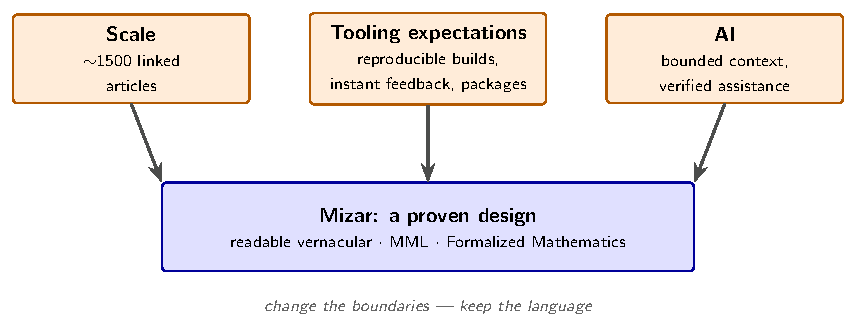
\includegraphics[width=\textwidth,height=0.52\textheight,keepaspectratio]{figures/three_pressures.pdf}
\end{center}
\begin{itemize}
\setlength{\itemsep}{1pt}
\setlength{\parsep}{0pt}
\setlength{\parskip}{0pt}
\item This diagram brings the three reasons together: library size, tools, and AI.
\item They do not mean that Mizar's design was wrong.
\item They explain why I want to update some boundaries while keeping Mizar's readable mathematical language.
\end{itemize}
\note{
\smallskip
\textbf{Read aloud:}
\begin{itemize}
\setlength{\itemsep}{1pt}
\setlength{\parsep}{0pt}
\setlength{\parskip}{0pt}
\item This diagram brings the three reasons together: library size, tools, and AI.
\item They do not mean that Mizar's design was wrong.
\item They explain why I want to update some boundaries while keeping Mizar's readable mathematical language.
\end{itemize}
}
\end{frame}

\begin{frame}[fragile,t]{1.6 - The Design Rule}
\smallskip
\textbf{Key Phrase:}
\begin{center}
\begin{beamercolorbox}[rounded=true,sep=2.5mm,wd=0.9\textwidth]{keyphrase}
\centering\itshape Do not make proofs harder to read to add automation.\\ Use automation to protect and extend readability.
\end{beamercolorbox}
\end{center}
\begin{itemize}
\setlength{\itemsep}{1pt}
\setlength{\parsep}{0pt}
\setlength{\parskip}{0pt}
\item This gives us three questions. Can people still read the proof? Can tools inspect its context? Will the design work as the library grows?
\item The next eight stories apply these questions to specific problems.
\end{itemize}
\smallskip
\textbf{Details for later review:}
\begin{footnotesize}
\setlength{\tabcolsep}{3pt}
\renewcommand{\arraystretch}{1.15}
\begin{tabularx}{\textwidth}{>{\raggedright\arraybackslash}X>{\raggedright\arraybackslash}X}
\toprule
\textbf{Goal} & \textbf{Test for every feature} \\
\midrule
Readability & does proof text still read as mathematics? \\
AI-readiness & can a tool see a limited context that we can audit? \\
Scalability & do boundaries stay stable as the library grows? \\
\bottomrule
\end{tabularx}
\end{footnotesize}

\note{
\smallskip
\textbf{Read aloud:}
\begin{itemize}
\setlength{\itemsep}{1pt}
\setlength{\parsep}{0pt}
\setlength{\parskip}{0pt}
\item Do not make proofs harder to read to add automation. Use automation to protect and extend readability.
\item This gives us three questions. Can people still read the proof? Can tools inspect its context? Will the design work as the library grows?
\item The next eight stories apply these questions to specific problems.
\end{itemize}
}
\end{frame}

\section{Part 2. Story 1: Dependencies You Can See}
\begin{frame}[fragile,t]{2.1 - The Problem}
\smallskip
\textbf{This environment lists dependencies}~\badgeMML
\begin{lstlisting}[language={mizar},basicstyle=\ttfamily\footnotesize]
environ

 vocabularies XBOOLE_0, SUBSET_1, BINOP_1, ZFMISC_1, STRUCT_0, ARYTM_3,
      FUNCT_1, FUNCT_5, SUPINF_2, ARYTM_1, RELAT_1, MESFUNC1, ALGSTR_0, CARD_1;
 notations TARSKI, XBOOLE_0, SUBSET_1, ZFMISC_1, BINOP_1, FUNCT_5, ORDINAL1,
      CARD_1, STRUCT_0;
 constructors BINOP_1, STRUCT_0, ZFMISC_1, FUNCT_5;
 registrations ZFMISC_1, CARD_1, STRUCT_0;
 theorems STRUCT_0;

begin :: Additive structures
\end{lstlisting}
\begin{itemize}
\setlength{\itemsep}{1pt}
\setlength{\parsep}{0pt}
\setlength{\parskip}{0pt}
\item Our first story is about dependencies. These lists tell Mizar which library material an article needs.
\item This form has supported library growth for decades. The question is how to make dependencies easier to review in a larger library.
\end{itemize}
\note{
\smallskip
\textbf{Read aloud:}
\begin{itemize}
\setlength{\itemsep}{1pt}
\setlength{\parsep}{0pt}
\setlength{\parskip}{0pt}
\item This environment lists dependencies.
\item Our first story is about dependencies. These lists tell Mizar which library material an article needs.
\item This form has supported library growth for decades. The question is how to make dependencies easier to review in a larger library.
\end{itemize}
\smallskip
\textbf{Optional notes and sources:}
\begin{itemize}
\setlength{\itemsep}{1pt}
\setlength{\parsep}{0pt}
\setlength{\parskip}{0pt}
\item Source: current MML \texttt{algstr\_0.miz}, lines 15-25.
\end{itemize}
}
\end{frame}

\begin{frame}[fragile,t]{2.2 - Why This Is Difficult\deepdivetag}
\smallskip
\textbf{Key Points:}
\begin{itemize}
\setlength{\itemsep}{1pt}
\setlength{\parsep}{0pt}
\setlength{\parskip}{0pt}
\item Information about a symbol's origin is spread across several role lists. A reviewer cannot see which article provides which notation, constructor, or cluster.
\item The Accommodator resolves the environment. But the resolved dependencies are not source text that a person can review.
\item Tools cannot cache or invalidate units smaller than an article.
\item Moving a theorem between articles risks breaking unknown dependents.
\end{itemize}
\smallskip
\textbf{Message:}
\begin{itemize}
\setlength{\itemsep}{1pt}
\setlength{\parsep}{0pt}
\setlength{\parskip}{0pt}
\item Implicit dependencies add work to every edit, review, and tool. That cost grows with the library.
\end{itemize}
\note{
\smallskip
\textbf{Read aloud:}
\begin{itemize}
\setlength{\itemsep}{1pt}
\setlength{\parsep}{0pt}
\setlength{\parskip}{0pt}
\item Information about a symbol's origin is spread across several role lists. A reviewer cannot see which article provides which notation, constructor, or cluster.
\item The Accommodator resolves the environment. But the resolved dependencies are not source text that a person can review.
\item Tools cannot cache or invalidate units smaller than an article.
\item Moving a theorem between articles risks breaking unknown dependents.
\item Implicit dependencies add work to every edit, review, and tool. That cost grows with the library.
\end{itemize}
}
\end{frame}

\begin{frame}[fragile,t]{2.3 - The Evo Answer: Import Prelude}
\smallskip
\textbf{Evo puts imports before definitions}~\badgeSpec
\begin{lstlisting}[language={mizar},basicstyle=\ttfamily\footnotesize]
import .function;
import mml.algebra.structure.sorted;

definition
  let S be 1-sorted;
  mode BinOpDef: BinOp of S is
    Function of [: S.carrier, S.carrier :], S.carrier;
end;
\end{lstlisting}
\begin{itemize}
\setlength{\itemsep}{1pt}
\setlength{\parsep}{0pt}
\setlength{\parskip}{0pt}
\item Here, the imports come before the first non-import item.
\item They provide the initial active lexicon. Local declarations extend it after their declaration points.
\item Imported items keep their source FQNs. Package and module paths give each item a stable fully-qualified name.
\end{itemize}
\note{
\smallskip
\textbf{Read aloud:}
\begin{itemize}
\setlength{\itemsep}{1pt}
\setlength{\parsep}{0pt}
\setlength{\parskip}{0pt}
\item Evo puts imports before definitions.
\item Here, the imports come before the first non-import item.
\item They provide the initial active lexicon. Local declarations extend it after their declaration points.
\item Imported items keep their source FQNs. Package and module paths give each item a stable fully-qualified name.
\end{itemize}
}
\end{frame}

\begin{frame}[fragile,t]{2.4 - The Evo Answer: Packages\deepdivetag}
\smallskip
\textbf{Mizar Evo}~\badgeSpec
\begin{lstlisting}[language={toml},basicstyle=\ttfamily\footnotesize]
[package]
name    = "algebra"
version = "2.3.1"
edition = "2025"

[dependencies]
mml_core = "^1.0"
topology = { version = "^0.9", features = ["metric"] }
\end{lstlisting}
\smallskip
\textbf{Key Points:}
\begin{itemize}
\setlength{\itemsep}{1pt}
\setlength{\parsep}{0pt}
\setlength{\parskip}{0pt}
\item reproducible builds need fixed source, lockfile, toolchain, and verifier settings, including deterministic ATP evidence;
\item versioned reuse (SemVer) replaces manual copying between article sets.
\end{itemize}
\note{
\smallskip
\textbf{Read aloud:}
\begin{itemize}
\setlength{\itemsep}{1pt}
\setlength{\parsep}{0pt}
\setlength{\parskip}{0pt}
\item reproducible builds need fixed source, lockfile, toolchain, and verifier settings, including deterministic ATP evidence;
\item versioned reuse (SemVer) replaces manual copying between article sets.
\end{itemize}
}
\end{frame}

\begin{frame}[fragile,t]{2.5 - Migrating The Environment\deepdivetag}
\begin{center}
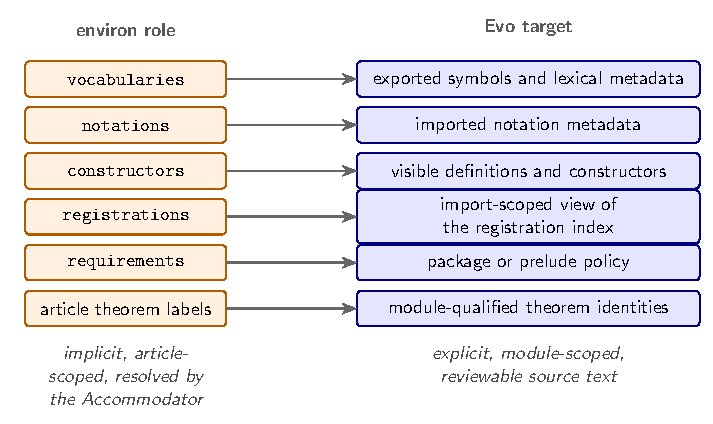
\includegraphics[width=\textwidth,height=0.63\textheight,keepaspectratio]{figures/environ_migration.pdf}
\end{center}
\smallskip
\textbf{Message:}
\begin{itemize}
\setlength{\itemsep}{1pt}
\setlength{\parsep}{0pt}
\setlength{\parskip}{0pt}
\item Migration changes more than names: reports must show each module's syntax, semantics, and automation.
\end{itemize}
\note{
\smallskip
\textbf{Read aloud:}
\begin{itemize}
\setlength{\itemsep}{1pt}
\setlength{\parsep}{0pt}
\setlength{\parskip}{0pt}
\item Migration changes more than names: reports must show each module's syntax, semantics, and automation.
\end{itemize}
}
\end{frame}

\begin{frame}[fragile,t]{2.6 - What Is Preserved, What We Ask}
\begin{itemize}
\setlength{\itemsep}{1pt}
\setlength{\parsep}{0pt}
\setlength{\parskip}{0pt}
\item The aim is to preserve the mathematics and theorem identities during migration.
\item A module is still a readable text, with article-style authorship.
\item Origin metadata records where migrated items came from. I will return to this when I discuss publication.
\item The questions below are for later review. I will now turn to structures.
\end{itemize}
\smallskip
\textbf{Questions for later review:}
\begin{itemize}
\setlength{\itemsep}{1pt}
\setlength{\parsep}{0pt}
\setlength{\parskip}{0pt}
\item Which \texttt{environ} roles must remain visually familiar during migration?
\item Which current article dependencies are hardest to explain, and would make the best test cases for generated dependency reports?
\end{itemize}
\note{
\smallskip
\textbf{Read aloud:}
\begin{itemize}
\setlength{\itemsep}{1pt}
\setlength{\parsep}{0pt}
\setlength{\parskip}{0pt}
\item The aim is to preserve the mathematics and theorem identities during migration.
\item A module is still a readable text, with article-style authorship.
\item Origin metadata records where migrated items came from. I will return to this when I discuss publication.
\item The questions below are for later review. I will now turn to structures.
\end{itemize}
}
\end{frame}

\section{Part 3. Story 2: Structures Without Hidden Merges}
\begin{frame}[fragile,t]{3.1 - The Problem}
\smallskip
\textbf{This structure uses the familiar compact form}~\badgeMML
\begin{lstlisting}[language={mizar},basicstyle=\ttfamily\footnotesize]
definition
  struct (1-sorted) addMagma (# carrier -> set, addF -> BinOp of the carrier
  #);
end;
\end{lstlisting}
\begin{itemize}
\setlength{\itemsep}{1pt}
\setlength{\parsep}{0pt}
\setlength{\parskip}{0pt}
\item One declaration contains the parent link, fields, and selectors.
\item With several parents, it also determines which inherited fields are shared.
\item Additive and multiplicative views depend on naming conventions.
\item The syntax does not separate stored data from canonical values such as zero.
\item Evo proposes a more explicit way to state these choices.
\end{itemize}
\note{
\smallskip
\textbf{Read aloud:}
\begin{itemize}
\setlength{\itemsep}{1pt}
\setlength{\parsep}{0pt}
\setlength{\parskip}{0pt}
\item This structure uses the familiar compact form.
\item One declaration contains the parent link, fields, and selectors.
\item With several parents, it also determines which inherited fields are shared.
\item Additive and multiplicative views depend on naming conventions.
\item The syntax does not separate stored data from canonical values such as zero.
\item Evo proposes a more explicit way to state these choices.
\end{itemize}
\smallskip
\textbf{Optional notes and sources:}
\begin{itemize}
\setlength{\itemsep}{1pt}
\setlength{\parsep}{0pt}
\setlength{\parskip}{0pt}
\item This short form keeps structures close to informal mathematical writing.
\item Source: current MML \texttt{algstr\_0.miz}, lines 37-40.
\end{itemize}
}
\end{frame}

\begin{frame}[fragile,t]{3.2 - Why This Is Difficult\deepdivetag}
\smallskip
\textbf{Key Points:}
\begin{itemize}
\setlength{\itemsep}{1pt}
\setlength{\parsep}{0pt}
\setlength{\parskip}{0pt}
\item With diamond inheritance, readers need to trace which inherited selectors are shared. Evo proposes explicit member mappings for these paths.
\item The syntax does not tell a migration tool whether a selector is intrinsic data, a canonical value with obligations, or an inherited view.
\item Errors appear far from their cause, as type mismatches in later articles.
\end{itemize}
\smallskip
\textbf{Message:}
\begin{itemize}
\setlength{\itemsep}{1pt}
\setlength{\parsep}{0pt}
\setlength{\parskip}{0pt}
\item At MML scale, structure inheritance is a graph maintenance problem, and the graph needs explicit edges that the verifier can check.
\end{itemize}
\note{
\smallskip
\textbf{Read aloud:}
\begin{itemize}
\setlength{\itemsep}{1pt}
\setlength{\parsep}{0pt}
\setlength{\parskip}{0pt}
\item With diamond inheritance, readers need to trace which inherited selectors are shared. Evo proposes explicit member mappings for these paths.
\item The syntax does not tell a migration tool whether a selector is intrinsic data, a canonical value with obligations, or an inherited view.
\item Errors appear far from their cause, as type mismatches in later articles.
\item At MML scale, structure inheritance is a graph maintenance problem, and the graph needs explicit edges that the verifier can check.
\end{itemize}
}
\end{frame}

\begin{frame}[fragile,t]{3.3 - The Evo Answer: Field, Property, Attribute}
\smallskip
\textbf{Evo separates fields, properties, and attributes}~\badgeSpec
\begin{lstlisting}[language={mizar},basicstyle=\ttfamily\small]
definition
  struct AddLoopStr where
    field carrier -> set;
    field add -> BinOp of carrier;
    property zero -> Element of carrier;
  end;
end;
\end{lstlisting}
\begin{itemize}
\setlength{\itemsep}{1pt}
\setlength{\parsep}{0pt}
\setlength{\parskip}{0pt}
\item A field stores data, like \texttt{carrier} and \texttt{add} here. Fields are constructor arguments and determine equality of exact instances.
\item A property, like \texttt{zero} here, gets its value from an implementation. The declaration alone supplies no value. \texttt{means} requires existence and uniqueness; \texttt{equals} gives a term.
\item An attribute is a predicate-style refinement. It supports cluster propagation and does not change the layout.
\end{itemize}
\note{
\smallskip
\textbf{Read aloud:}
\begin{itemize}
\setlength{\itemsep}{1pt}
\setlength{\parsep}{0pt}
\setlength{\parskip}{0pt}
\item Evo separates fields, properties, and attributes.
\item A field stores data, like \texttt{carrier} and \texttt{add} here. Fields are constructor arguments and determine equality of exact instances.
\item A property, like \texttt{zero} here, gets its value from an implementation. The declaration alone supplies no value. \texttt{means} requires existence and uniqueness; \texttt{equals} gives a term.
\item An attribute is a predicate-style refinement. It supports cluster propagation and does not change the layout.
\end{itemize}
\smallskip
\textbf{Optional notes and sources:}
\begin{itemize}
\setlength{\itemsep}{1pt}
\setlength{\parsep}{0pt}
\setlength{\parskip}{0pt}
\item Overlapping property implementations need \texttt{coherence}.
\end{itemize}
}
\end{frame}

\begin{frame}[fragile,t]{3.4 - The Evo Answer: Explicit Inheritance}
\smallskip
\textbf{Evo writes each parent mapping explicitly}~\badgeSpec
\begin{lstlisting}[language={mizar},basicstyle=\ttfamily\footnotesize]
definition
  struct AddMagma where
    field carrier -> set;
    field add -> BinOp of carrier;
  end;

  inherit AddMagma extends Magma where
    field carrier from carrier;
    field add from binop;    :: renamed
  end;
end;
\end{lstlisting}
\begin{itemize}
\setlength{\itemsep}{1pt}
\setlength{\parsep}{0pt}
\setlength{\parskip}{0pt}
\item There is one \texttt{inherit} statement for each parent.
\item Here, \texttt{from} maps the child's \texttt{add} field to the parent's \texttt{binop} field.
\item Syntactically identical member types need no proof, even if a name changes. Other types need \texttt{coherence} proofs of subtype inclusion.
\end{itemize}
\note{
\smallskip
\textbf{Read aloud:}
\begin{itemize}
\setlength{\itemsep}{1pt}
\setlength{\parsep}{0pt}
\setlength{\parskip}{0pt}
\item Evo writes each parent mapping explicitly.
\item There is one \texttt{inherit} statement for each parent.
\item Here, \texttt{from} maps the child's \texttt{add} field to the parent's \texttt{binop} field.
\item Syntactically identical member types need no proof, even if a name changes. Other types need \texttt{coherence} proofs of subtype inclusion.
\end{itemize}
}
\end{frame}

\begin{frame}[fragile,t]{3.5 - The Evo Answer: Diamonds Become Checkable (1/2)}
\smallskip
\textbf{This child has two parent structures}~\badgeSpec
\begin{lstlisting}[language={mizar},basicstyle=\ttfamily\footnotesize]
definition
  struct DoubleLoopStr where
    field carrier -> set;
    field add -> BinOp of carrier;
    field mul -> BinOp of carrier;
    property zero -> Element of carrier;
    property one -> Element of carrier;
  end;

  inherit DoubleLoopStr extends AddLoopStr;
  inherit DoubleLoopStr extends MulLoopStr;
end;
\end{lstlisting}
\note{
\smallskip
\textbf{Read aloud:}
\begin{itemize}
\setlength{\itemsep}{1pt}
\setlength{\parsep}{0pt}
\setlength{\parskip}{0pt}
\item This child has two parent structures.
\end{itemize}
\smallskip
\textbf{Optional notes and sources:}
\begin{itemize}
\setlength{\itemsep}{1pt}
\setlength{\parsep}{0pt}
\setlength{\parskip}{0pt}
\item The diagram assumes the shown mappings from \texttt{AddLoopStr} and \texttt{MulLoopStr} to \texttt{Magma}. The code adds their shared child, \texttt{DoubleLoopStr}.
\end{itemize}
}
\end{frame}

\begin{frame}[fragile,t]{3.5 - The Evo Answer: Diamonds Become Checkable (2/2)}
\smallskip
\textbf{The diagram shows the inheritance paths}~\badgeSketch
\begin{center}
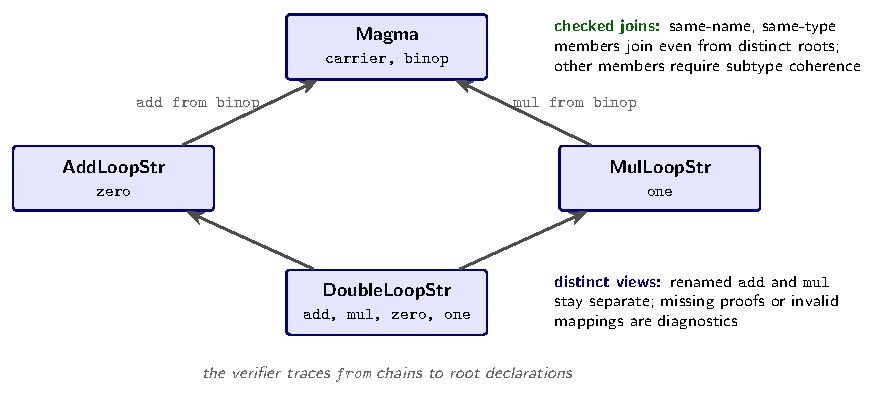
\includegraphics[width=\textwidth,height=0.57\textheight,keepaspectratio]{figures/diamond_inheritance.pdf}
\end{center}
\begin{itemize}
\setlength{\itemsep}{1pt}
\setlength{\parsep}{0pt}
\setlength{\parskip}{0pt}
\item Same-name, same-type members can join across roots. Different member types need \texttt{coherence} proofs of subtype inclusion.
\item Renamed views stay distinct. Invalid mappings or missing proofs give diagnostics.
\end{itemize}
\note{
\smallskip
\textbf{Read aloud:}
\begin{itemize}
\setlength{\itemsep}{1pt}
\setlength{\parsep}{0pt}
\setlength{\parskip}{0pt}
\item The diagram shows the inheritance paths.
\item Same-name, same-type members can join across roots. Different member types need \texttt{coherence} proofs of subtype inclusion.
\item Renamed views stay distinct. Invalid mappings or missing proofs give diagnostics.
\end{itemize}
}
\end{frame}

\begin{frame}[fragile,t]{3.6 - What Is Preserved, What We Ask}
\begin{itemize}
\setlength{\itemsep}{1pt}
\setlength{\parsep}{0pt}
\setlength{\parskip}{0pt}
\item We still use carriers, selectors, and \texttt{Element of}, as in Mizar.
\item Aggregates become longer only when we need to make a hidden choice explicit.
\item The main question is whether this form is readable in real algebraic articles.
\item I would like to test it on structures with several inheritance paths. Next, I will discuss registrations and clusters.
\end{itemize}
\smallskip
\textbf{Questions for later review:}
\begin{itemize}
\setlength{\itemsep}{1pt}
\setlength{\parsep}{0pt}
\setlength{\parskip}{0pt}
\item Is the \texttt{field} / \texttt{property} / \texttt{attribute} split readable in real algebraic articles, or does it require too many annotations in simple cases?
\item Is one-parent-per-\texttt{inherit} acceptable for parts of MML with much inheritance, such as the \texttt{ALGSTR} and topology hierarchies?
\item Which MML structures would be the best diamond test cases?
\end{itemize}
\note{
\smallskip
\textbf{Read aloud:}
\begin{itemize}
\setlength{\itemsep}{1pt}
\setlength{\parsep}{0pt}
\setlength{\parskip}{0pt}
\item We still use carriers, selectors, and \texttt{Element of}, as in Mizar.
\item Aggregates become longer only when we need to make a hidden choice explicit.
\item The main question is whether this form is readable in real algebraic articles.
\item I would like to test it on structures with several inheritance paths. Next, I will discuss registrations and clusters.
\end{itemize}
}
\end{frame}

\section{Part 4. Story 3: Automation You Can Audit}
\begin{frame}[fragile,t]{4.1 - The Problem}
\smallskip
\textbf{This registration lets Mizar reuse a proved fact}~\badgeMML
\begin{lstlisting}[language={mizar},basicstyle=\ttfamily\small]
registration
  let M be addMagma;
  cluster right_add-cancelable left_add-cancelable -> add-cancelable for
Element
    of M;
  coherence;
end;
\end{lstlisting}
\begin{itemize}
\setlength{\itemsep}{1pt}
\setlength{\parsep}{0pt}
\setlength{\parskip}{0pt}
\item Registrations let attributes propagate automatically, so proofs stay short.
\item I want to keep this idea and make the steps of the automation easier to see.
\end{itemize}
\note{
\smallskip
\textbf{Read aloud:}
\begin{itemize}
\setlength{\itemsep}{1pt}
\setlength{\parsep}{0pt}
\setlength{\parskip}{0pt}
\item This registration lets Mizar reuse a proved fact.
\item Registrations let attributes propagate automatically, so proofs stay short.
\item I want to keep this idea and make the steps of the automation easier to see.
\end{itemize}
\smallskip
\textbf{Optional notes and sources:}
\begin{itemize}
\setlength{\itemsep}{1pt}
\setlength{\parsep}{0pt}
\setlength{\parskip}{0pt}
\item Source: current MML \texttt{algstr\_0.miz}, lines 104-109.
\end{itemize}
}
\end{frame}

\begin{frame}[fragile,t]{4.2 - Why This Is Difficult\deepdivetag}
\smallskip
\textbf{Key Points:}
\begin{itemize}
\setlength{\itemsep}{1pt}
\setlength{\parsep}{0pt}
\setlength{\parskip}{0pt}
\item When a proof fails, "why does the checker not see that this is a Group?" has no local answer. The cause is somewhere in the environment.
\item Users cannot see which registrations fired or in which order. The automation is powerful, but explaining it becomes harder as it does more.
\item For an AI assistant the situation is worse: it must guess the cluster state instead of reading it.
\end{itemize}
\smallskip
\textbf{Message:}
\begin{itemize}
\setlength{\itemsep}{1pt}
\setlength{\parsep}{0pt}
\setlength{\parskip}{0pt}
\item Automation without explanations makes a large library harder to maintain, even when it is sound.
\end{itemize}
\note{
\smallskip
\textbf{Read aloud:}
\begin{itemize}
\setlength{\itemsep}{1pt}
\setlength{\parsep}{0pt}
\setlength{\parskip}{0pt}
\item When a proof fails, "why does the checker not see that this is a Group?" has no local answer. The cause is somewhere in the environment.
\item Users cannot see which registrations fired or in which order. The automation is powerful, but explaining it becomes harder as it does more.
\item For an AI assistant the situation is worse: it must guess the cluster state instead of reading it.
\item Automation without explanations makes a large library harder to maintain, even when it is sound.
\end{itemize}
}
\end{frame}

\begin{frame}[fragile,t]{4.3 - The Evo Answer: Labeled, Traceable Registrations}
\smallskip
\textbf{Evo gives every registration item a label}~\badgeSpec
\begin{lstlisting}[language={mizar},basicstyle=\ttfamily\small]
registration
  cluster EmptyImpliesFinite: empty -> finite for set;
  coherence proof ... end;

  cluster FiniteImpliesCountable: finite -> countable for set;
  coherence proof ... end;
end;
\end{lstlisting}
\begin{itemize}
\setlength{\itemsep}{1pt}
\setlength{\parsep}{0pt}
\setlength{\parskip}{0pt}
\item We can cite the label in \texttt{by}. It also appears in diagnostics and the module interface.
\item The verifier uses an import-filtered view of the global cluster graph.
\item \texttt{explain-attribute} and resolution traces explain success or failure. For example, they can show the steps from empty to finite to countable.
\end{itemize}
\note{
\smallskip
\textbf{Read aloud:}
\begin{itemize}
\setlength{\itemsep}{1pt}
\setlength{\parsep}{0pt}
\setlength{\parskip}{0pt}
\item Evo gives every registration item a label.
\item We can cite the label in \texttt{by}. It also appears in diagnostics and the module interface.
\item The verifier uses an import-filtered view of the global cluster graph.
\item \texttt{explain-attribute} and resolution traces explain success or failure. For example, they can show the steps from empty to finite to countable.
\end{itemize}
}
\end{frame}

\begin{frame}[fragile,t]{4.4 - The Evo Answer: Oriented Reductions\deepdivetag}
\smallskip
\textbf{Mizar Evo}~\badgeSpec
\begin{lstlisting}[language={mizar},basicstyle=\ttfamily\footnotesize]
registration
  let n be Nat;
  reduce NatAddZero: n + 0 to n;
  reducibility
  proof
    let n be Nat;
    thus n + 0 = n by mml.number.natural.Nat_add_zero;
  end;
end;
\end{lstlisting}
\smallskip
\textbf{Key Points:}
\begin{itemize}
\setlength{\itemsep}{1pt}
\setlength{\parsep}{0pt}
\setlength{\parskip}{0pt}
\item a reduction is an oriented simplification backed by an equality proof;
\item the right side must be strictly smaller, so imported rules cannot loop, and rule selection is deterministic (pattern subsumption, then guard specificity, then FQN tie-break);
\item unoriented identification idioms become auditable \texttt{reduce} items.
\end{itemize}
\note{
\smallskip
\textbf{Read aloud:}
\begin{itemize}
\setlength{\itemsep}{1pt}
\setlength{\parsep}{0pt}
\setlength{\parskip}{0pt}
\item a reduction is an oriented simplification backed by an equality proof;
\item the right side must be strictly smaller, so imported rules cannot loop, and rule selection is deterministic (pattern subsumption, then guard specificity, then FQN tie-break);
\item unoriented identification idioms become auditable \texttt{reduce} items.
\end{itemize}
}
\end{frame}

\begin{frame}[fragile,t]{4.5 - What Is Preserved, What We Ask}
\begin{itemize}
\setlength{\itemsep}{1pt}
\setlength{\parsep}{0pt}
\setlength{\parskip}{0pt}
\item Registrations and clusters remain part of the language, and proofs stay short.
\item Applying a cluster does not require us to repeat its proof.
\item A reduction simplifies a term using an equality. It may need local guard evidence or an explicit equality citation.
\item I would like to learn which explanations would help most in daily MML work. This leads to the next story: stronger proof search.
\end{itemize}
\smallskip
\textbf{Questions for later review:}
\begin{itemize}
\setlength{\itemsep}{1pt}
\setlength{\parsep}{0pt}
\setlength{\parskip}{0pt}
\item Which cluster explanations would help most with daily work: failure explanations, firing traces, or difference reports between environments?
\item Which MML article families make the most complex use of registrations and should become migration benchmarks for the cluster graph?
\end{itemize}
\note{
\smallskip
\textbf{Read aloud:}
\begin{itemize}
\setlength{\itemsep}{1pt}
\setlength{\parsep}{0pt}
\setlength{\parskip}{0pt}
\item Registrations and clusters remain part of the language, and proofs stay short.
\item Applying a cluster does not require us to repeat its proof.
\item A reduction simplifies a term using an equality. It may need local guard evidence or an explicit equality citation.
\item I would like to learn which explanations would help most in daily MML work. This leads to the next story: stronger proof search.
\end{itemize}
}
\end{frame}

\section{Part 5. Story 4: Powerful Search, Small Trust}
\begin{frame}[fragile,t]{5.1 - The Problem}
\begin{itemize}
\setlength{\itemsep}{1pt}
\setlength{\parsep}{0pt}
\setlength{\parskip}{0pt}
\item Users want stronger automation, including larger \texttt{by} steps and hammer-style search.
\item MizAR and MPTP already use ATP search with MML premises.
\item Evo's goal is to keep proof checking small as search becomes stronger.
\item A search result alone is not a kernel-verified proof. We need checkable evidence.
\item So the question is this.
\end{itemize}
\smallskip
\textbf{Key Phrase:}
\begin{center}
\begin{beamercolorbox}[rounded=true,sep=2.5mm,wd=0.9\textwidth]{keyphrase}
\centering\itshape How do we get modern proof search\\ without trusting the searcher?
\end{beamercolorbox}
\end{center}
\note{
\smallskip
\textbf{Read aloud:}
\begin{itemize}
\setlength{\itemsep}{1pt}
\setlength{\parsep}{0pt}
\setlength{\parskip}{0pt}
\item Users want stronger automation, including larger \texttt{by} steps and hammer-style search.
\item MizAR and MPTP already use ATP search with MML premises.
\item Evo's goal is to keep proof checking small as search becomes stronger.
\item A search result alone is not a kernel-verified proof. We need checkable evidence.
\item So the question is this.
\item How do we get modern proof search without trusting the searcher?
\end{itemize}
\smallskip
\textbf{Optional notes and sources:}
\begin{itemize}
\setlength{\itemsep}{1pt}
\setlength{\parsep}{0pt}
\setlength{\parskip}{0pt}
\item This builds on MizAR, MPTP, and hammer research. I am describing Evo's evidence contract, not making a claim that earlier tools must trust their search backends.
\end{itemize}
}
\end{frame}

\begin{frame}[fragile,t]{5.2 - The Evo Answer: A Reasoning Boundary}
\begin{center}
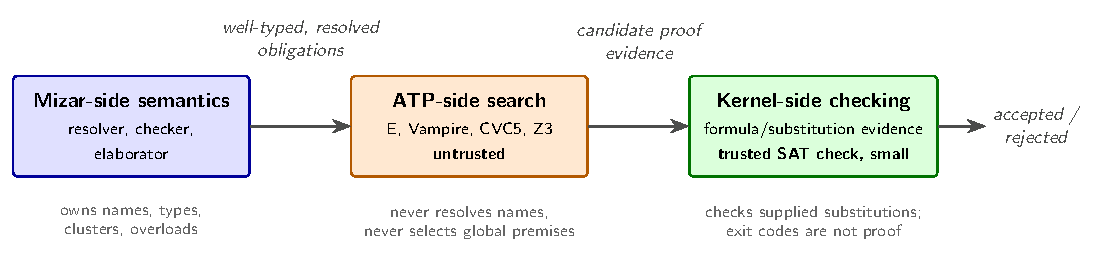
\includegraphics[width=\textwidth,height=0.52\textheight,keepaspectratio]{figures/reasoning_boundary.pdf}
\end{center}
\begin{itemize}
\setlength{\itemsep}{1pt}
\setlength{\parsep}{0pt}
\setlength{\parskip}{0pt}
\item We can read this diagram from left to right.
\item Mizar-side phases resolve names, infer types, expand clusters, and pick overloads. ATPs do none of these tasks.
\item The kernel checks the supplied formulas and substitutions, then runs its trusted SAT check. It does not select premises or invent substitutions.
\item Earlier deterministic discharge also needs replayable evidence.
\end{itemize}
\note{
\smallskip
\textbf{Read aloud:}
\begin{itemize}
\setlength{\itemsep}{1pt}
\setlength{\parsep}{0pt}
\setlength{\parskip}{0pt}
\item We can read this diagram from left to right.
\item Mizar-side phases resolve names, infer types, expand clusters, and pick overloads. ATPs do none of these tasks.
\item The kernel checks the supplied formulas and substitutions, then runs its trusted SAT check. It does not select premises or invent substitutions.
\item Earlier deterministic discharge also needs replayable evidence.
\end{itemize}
\smallskip
\textbf{Optional notes and sources:}
\begin{itemize}
\setlength{\itemsep}{1pt}
\setlength{\parsep}{0pt}
\setlength{\parskip}{0pt}
\item Development policy may record \texttt{externally\_attested} results. These are separate from kernel-verified proofs.
\end{itemize}
}
\end{frame}

\begin{frame}[fragile,t]{5.3 - Formula And Substitution Evidence}
\begin{center}
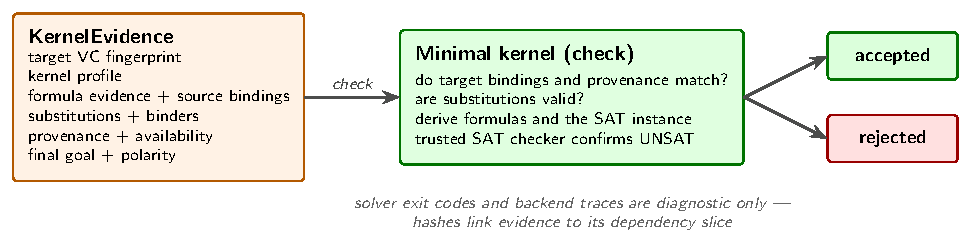
\includegraphics[width=\textwidth,height=0.52\textheight,keepaspectratio]{figures/certificate_replay.pdf}
\end{center}
\begin{itemize}
\setlength{\itemsep}{1pt}
\setlength{\parsep}{0pt}
\setlength{\parskip}{0pt}
\item Here we can see what the evidence contains: source formulas, substitutions, provenance, and target and goal bindings.
\item The kernel checks it, derives instantiated formulas and SAT clauses, and requires UNSAT from its trusted in-process Rust SAT checker.
\item Backend resolution traces, SMT proof objects, logs, and exit codes are not trusted acceptance evidence.
\end{itemize}
\note{
\smallskip
\textbf{Read aloud:}
\begin{itemize}
\setlength{\itemsep}{1pt}
\setlength{\parsep}{0pt}
\setlength{\parskip}{0pt}
\item Here we can see what the evidence contains: source formulas, substitutions, provenance, and target and goal bindings.
\item The kernel checks it, derives instantiated formulas and SAT clauses, and requires UNSAT from its trusted in-process Rust SAT checker.
\item Backend resolution traces, SMT proof objects, logs, and exit codes are not trusted acceptance evidence.
\end{itemize}
\smallskip
\textbf{Optional notes and sources:}
\begin{itemize}
\setlength{\itemsep}{1pt}
\setlength{\parsep}{0pt}
\setlength{\parskip}{0pt}
\item Hashes bind evidence to its dependency context. The kernel also checks binder conditions and the goal's refutation polarity.
\end{itemize}
}
\end{frame}

\begin{frame}[fragile,t]{5.4 - The Same Boundary Controls AI}
\smallskip
\textbf{An AI tool could help repair a citation like this one}~\badgeMML
\begin{lstlisting}[language={mizar},basicstyle=\ttfamily\small]
theorem
  for F being non degenerated ZeroOneStr holds 1.F in NonZero F
proof
  let F be non degenerated ZeroOneStr;
  not 1.F in {0.F} by TARSKI:def 1;
  hence thesis by XBOOLE_0:def 5;
end;
\end{lstlisting}
\begin{itemize}
\setlength{\itemsep}{1pt}
\setlength{\parsep}{0pt}
\setlength{\parskip}{0pt}
\item The AI tool can propose a missing or more precise \texttt{by} reference.
\item This is a local edit that keeps the statement's meaning.
\item The verifier checks it just as it would check a human edit.
\item The AI proposes the change. The verifier and kernel decide whether to accept it.
\end{itemize}
\note{
\smallskip
\textbf{Read aloud:}
\begin{itemize}
\setlength{\itemsep}{1pt}
\setlength{\parsep}{0pt}
\setlength{\parskip}{0pt}
\item An AI tool could help repair a citation like this one.
\item The AI tool can propose a missing or more precise \texttt{by} reference.
\item This is a local edit that keeps the statement's meaning.
\item The verifier checks it just as it would check a human edit.
\item The AI proposes the change. The verifier and kernel decide whether to accept it.
\end{itemize}
\smallskip
\textbf{Optional notes and sources:}
\begin{itemize}
\setlength{\itemsep}{1pt}
\setlength{\parsep}{0pt}
\setlength{\parskip}{0pt}
\item The assistant's strength never enters the trusted base.
\item Source: current MML \texttt{struct\_0.miz}, lines 637-643.
\end{itemize}
}
\end{frame}

\begin{frame}[fragile,t]{5.5 - Edit Classes: Green, Yellow, Red\deepdivetag}
\begin{footnotesize}
\setlength{\tabcolsep}{3pt}
\renewcommand{\arraystretch}{1.15}
\begin{tabularx}{\textwidth}{>{\raggedright\arraybackslash}X>{\raggedright\arraybackslash}X>{\raggedright\arraybackslash}X}
\toprule
\textbf{Class} & \textbf{Examples} & \textbf{Policy} \\
\midrule
Green & add citation, insert \texttt{qua}, info annotation & can be proposed automatically; still verified \\
Yellow & add import, local lemma, registration & proposed with human review \\
Red & weaken theorem, change definition, add axiom & forbidden to ordinary agents \\
\bottomrule
\end{tabularx}
\end{footnotesize}

\smallskip
\textbf{Forbidden repair}~\badgeSketch
\begin{lstlisting}[language={mizar},basicstyle=\ttfamily\small]
theorem
  for x be Nat holds x + 0 = x or x = 0;
\end{lstlisting}
\smallskip
\textbf{Message:}
\begin{itemize}
\setlength{\itemsep}{1pt}
\setlength{\parsep}{0pt}
\setlength{\parskip}{0pt}
\item Weakening a statement to make its proof easier is a Red edit; at most an agent may flag it for explicit human unsafe-edit review.
\end{itemize}
\note{
\smallskip
\textbf{Read aloud:}
\begin{itemize}
\setlength{\itemsep}{1pt}
\setlength{\parsep}{0pt}
\setlength{\parskip}{0pt}
\item Weakening a statement to make its proof easier is a Red edit; at most an agent may flag it for explicit human unsafe-edit review.
\end{itemize}
}
\end{frame}

\begin{frame}[fragile,t]{5.6 - What Is Preserved, What We Ask}
\begin{itemize}
\setlength{\itemsep}{1pt}
\setlength{\parsep}{0pt}
\setlength{\parskip}{0pt}
\item This keeps the de Bruijn discipline: a small trusted core checks acceptance. In this design, the core includes its SAT checker.
\item Proof text stays declarative and readable. Automation helps maintain the argument.
\item I would welcome your views on the evidence format.
\item Now let us look at the cost of checking a large library.
\end{itemize}
\smallskip
\textbf{Questions for later review:}
\begin{itemize}
\setlength{\itemsep}{1pt}
\setlength{\parsep}{0pt}
\setlength{\parskip}{0pt}
\item Is the formula/substitution evidence approach convincing for Mizar-style obligations, including clusters and definitional expansions?
\item Which evidence format would the team be most willing to audit?
\end{itemize}
\note{
\smallskip
\textbf{Read aloud:}
\begin{itemize}
\setlength{\itemsep}{1pt}
\setlength{\parsep}{0pt}
\setlength{\parskip}{0pt}
\item This keeps the de Bruijn discipline: a small trusted core checks acceptance. In this design, the core includes its SAT checker.
\item Proof text stays declarative and readable. Automation helps maintain the argument.
\item I would welcome your views on the evidence format.
\item Now let us look at the cost of checking a large library.
\end{itemize}
}
\end{frame}

\section{Part 6. Story 5: Verification That Scales}
\begin{frame}[fragile,t]{6.1 - The Problem}
\begin{itemize}
\setlength{\itemsep}{1pt}
\setlength{\parsep}{0pt}
\setlength{\parskip}{0pt}
\item Checking the whole MML takes hours.
\item The accepted article is the unit of reuse. A small edit can therefore cause more checking than we would like.
\item Memory use follows the article environment, including material outside the interface actually used.
\item These costs follow from the article as a unit. Evo proposes smaller units of reuse.
\end{itemize}
\note{
\smallskip
\textbf{Read aloud:}
\begin{itemize}
\setlength{\itemsep}{1pt}
\setlength{\parsep}{0pt}
\setlength{\parskip}{0pt}
\item Checking the whole MML takes hours.
\item The accepted article is the unit of reuse. A small edit can therefore cause more checking than we would like.
\item Memory use follows the article environment, including material outside the interface actually used.
\item These costs follow from the article as a unit. Evo proposes smaller units of reuse.
\end{itemize}
}
\end{frame}

\begin{frame}[fragile,t]{6.2 - The Evo Answer: Fingerprints And Incrementality (1/2)}
\begin{itemize}
\setlength{\itemsep}{1pt}
\setlength{\parsep}{0pt}
\setlength{\parskip}{0pt}
\item Evo uses fingerprints to decide when earlier results can be reused.
\item All relevant cache keys must match. Missing data causes a cache miss.
\item A proof-body edit does not rebuild importers when the exported statement and accepted status stay unchanged.
\item Independent modules, obligations, ATP runs, and kernel checks can run in parallel. Results are published in canonical order.
\end{itemize}
\note{
\smallskip
\textbf{Read aloud:}
\begin{itemize}
\setlength{\itemsep}{1pt}
\setlength{\parsep}{0pt}
\setlength{\parskip}{0pt}
\item Evo uses fingerprints to decide when earlier results can be reused.
\item All relevant cache keys must match. Missing data causes a cache miss.
\item A proof-body edit does not rebuild importers when the exported statement and accepted status stay unchanged.
\item Independent modules, obligations, ATP runs, and kernel checks can run in parallel. Results are published in canonical order.
\end{itemize}
\smallskip
\textbf{Optional notes and sources:}
\begin{itemize}
\setlength{\itemsep}{1pt}
\setlength{\parsep}{0pt}
\setlength{\parskip}{0pt}
\item The cache keys cover source, dependency slices, package and lockfile, toolchain, schema, policy, registrations, obligations, evidence, and witnesses.
\end{itemize}
}
\end{frame}

\begin{frame}[fragile,t]{6.2 - The Evo Answer: Fingerprints And Incrementality (2/2)}
\begin{center}
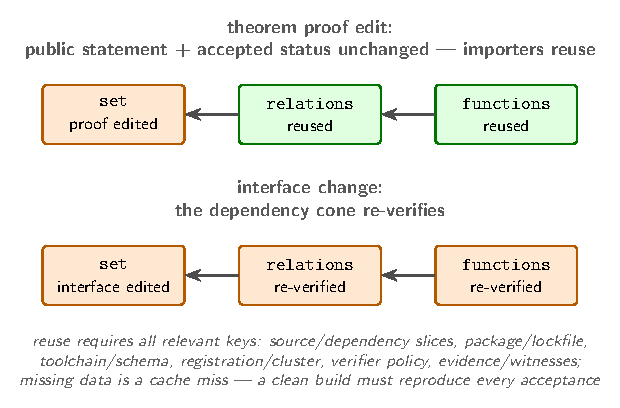
\includegraphics[width=\textwidth,height=0.52\textheight,keepaspectratio]{figures/fingerprint_graph.pdf}
\end{center}
\begin{center}
\begin{beamercolorbox}[rounded=true,sep=2.5mm,wd=0.9\textwidth]{keyphrase}
\centering\itshape Cache reuse is never proof authority.\\ A clean build must reproduce every acceptance.
\end{beamercolorbox}
\end{center}
\note{
\smallskip
\textbf{Read aloud:}
\begin{itemize}
\setlength{\itemsep}{1pt}
\setlength{\parsep}{0pt}
\setlength{\parskip}{0pt}
\item Cache reuse is never proof authority. A clean build must reproduce every acceptance.
\end{itemize}
}
\end{frame}

\begin{frame}[fragile,t]{6.3 - The Evo Answer: A Memory Contract\deepdivetag}
\begin{lstlisting}[language={},basicstyle=\ttfamily\footnotesize]
resident memory should scale with:
  active source and typed AST
  imported public interfaces
  import-filtered indexes
  active module obligations
  in-flight proof checks and ATP runs
  small caches

not with:
  imported proof bodies
  imported proof witnesses
  private lemmas outside the interface
  registration data outside the import closure
\end{lstlisting}
\smallskip
\textbf{Message:}
\begin{itemize}
\setlength{\itemsep}{1pt}
\setlength{\parsep}{0pt}
\setlength{\parskip}{0pt}
\item This is a resident-memory model, not a measured performance guarantee. Proof bodies and traces load lazily for specific queries.
\end{itemize}
\note{
\smallskip
\textbf{Read aloud:}
\begin{itemize}
\setlength{\itemsep}{1pt}
\setlength{\parsep}{0pt}
\setlength{\parskip}{0pt}
\item This is a resident-memory model, not a measured performance guarantee. Proof bodies and traces load lazily for specific queries.
\end{itemize}
}
\end{frame}

\begin{frame}[fragile,t]{6.4 - What Is Preserved, What We Ask}
\begin{itemize}
\setlength{\itemsep}{1pt}
\setlength{\parsep}{0pt}
\setlength{\parskip}{0pt}
\item Caching and parallel work change checking time. They must not change truth.
\item A person still reviews complete source text, in the style of an article.
\item We need tests that compare incremental results with a clean build.
\item I would like to use real MML maintenance tasks for these tests. Next, I will turn to templates.
\end{itemize}
\smallskip
\textbf{Questions for later review:}
\begin{itemize}
\setlength{\itemsep}{1pt}
\setlength{\parsep}{0pt}
\setlength{\parskip}{0pt}
\item What clean-build equivalence tests would make incremental verification trustworthy to the team that maintains MML today?
\item Which current maintenance operations (revisions, renamings) should we benchmark for incremental cost?
\end{itemize}
\note{
\smallskip
\textbf{Read aloud:}
\begin{itemize}
\setlength{\itemsep}{1pt}
\setlength{\parsep}{0pt}
\setlength{\parskip}{0pt}
\item Caching and parallel work change checking time. They must not change truth.
\item A person still reviews complete source text, in the style of an article.
\item We need tests that compare incremental results with a clean build.
\item I would like to use real MML maintenance tasks for these tests. Next, I will turn to templates.
\end{itemize}
}
\end{frame}

\section{Part 7. Story 6: Templates For Generic Mathematics}
\begin{frame}[fragile,t]{7.1 - The Problem, Part One: Schemes Use Separate Rules}
\smallskip
\textbf{This familiar scheme expresses induction}~\badgeMML
\begin{lstlisting}[language={mizar},basicstyle=\ttfamily\small]
scheme
  NatInd { P[Nat] } : for k being Nat holds P[k]
provided
A1: P[0] and
A2: for k be Nat st P[k] holds P[k + 1]
\end{lstlisting}
\begin{itemize}
\setlength{\itemsep}{1pt}
\setlength{\parsep}{0pt}
\setlength{\parskip}{0pt}
\item Schemes support second-order patterns such as induction, separation, and replacement.
\item Classic \texttt{scheme} blocks define theorem schemas. Parameterized definitions use other language forms.
\item Evo proposes a common template system for these tasks.
\end{itemize}
\note{
\smallskip
\textbf{Read aloud:}
\begin{itemize}
\setlength{\itemsep}{1pt}
\setlength{\parsep}{0pt}
\setlength{\parskip}{0pt}
\item This familiar scheme expresses induction.
\item Schemes support second-order patterns such as induction, separation, and replacement.
\item Classic \texttt{scheme} blocks define theorem schemas. Parameterized definitions use other language forms.
\item Evo proposes a common template system for these tasks.
\end{itemize}
\smallskip
\textbf{Optional notes and sources:}
\begin{itemize}
\setlength{\itemsep}{1pt}
\setlength{\parsep}{0pt}
\setlength{\parskip}{0pt}
\item Source: current MML \texttt{nat\_1.miz}, near line 90 (checked July 2, 2026).
\end{itemize}
}
\end{frame}

\begin{frame}[fragile,t]{7.2 - The Problem, Part Two: A Common Template System}
\begin{itemize}
\setlength{\itemsep}{1pt}
\setlength{\parsep}{0pt}
\setlength{\parskip}{0pt}
\item Mizar already has parameterized constructions, such as \texttt{Polynom-Ring L}.
\item The aim is to give definitions and theorem schemas a common template system.
\item Each kind of parameter still has explicit rules.
\item We need migration examples to see whether these rules make generic mathematics easier to write and maintain.
\end{itemize}
Source: POLYNOM3, definition 10 (\url{https://mizar.uwb.edu.pl/version/current/html/polynom3.html}).

\note{
\smallskip
\textbf{Read aloud:}
\begin{itemize}
\setlength{\itemsep}{1pt}
\setlength{\parsep}{0pt}
\setlength{\parskip}{0pt}
\item Mizar already has parameterized constructions, such as \texttt{Polynom-Ring L}.
\item The aim is to give definitions and theorem schemas a common template system.
\item Each kind of parameter still has explicit rules.
\item We need migration examples to see whether these rules make generic mathematics easier to write and maintain.
\end{itemize}
\smallskip
\textbf{Optional notes and sources:}
\begin{itemize}
\setlength{\itemsep}{1pt}
\setlength{\parsep}{0pt}
\setlength{\parskip}{0pt}
\item Source: POLYNOM3, definition 10 (\url{https://mizar.uwb.edu.pl/version/current/html/polynom3.html}).
\end{itemize}
}
\end{frame}

\begin{frame}[fragile,t]{7.3 - The Evo Answer: Templates}
\smallskip
\textbf{This template begins with a type parameter}~\badgeSpec
\begin{lstlisting}[language={mizar},basicstyle=\ttfamily\small]
definition
  let T be type;
  struct MagmaStr[T] where
    field carrier -> T;
    field binop -> BinOp of T;
  end;
end;
\end{lstlisting}
\begin{itemize}
\setlength{\itemsep}{1pt}
\setlength{\parsep}{0pt}
\setlength{\parskip}{0pt}
\item A template is an ordinary \texttt{definition} block. Its leading \texttt{let} binds the parameters.
\item Parameters can be types, values, predicates, or functors.
\item Predicate and functor parameters cannot occur in \texttt{attr}, \texttt{mode}, \texttt{struct}, \texttt{func}, or \texttt{pred} items.
\item Some templates allow short forms such as \texttt{Module over R} and \texttt{Subset of X}. Constrained templates require brackets.
\end{itemize}
\note{
\smallskip
\textbf{Read aloud:}
\begin{itemize}
\setlength{\itemsep}{1pt}
\setlength{\parsep}{0pt}
\setlength{\parskip}{0pt}
\item This template begins with a type parameter.
\item A template is an ordinary \texttt{definition} block. Its leading \texttt{let} binds the parameters.
\item Parameters can be types, values, predicates, or functors.
\item Predicate and functor parameters cannot occur in \texttt{attr}, \texttt{mode}, \texttt{struct}, \texttt{func}, or \texttt{pred} items.
\item Some templates allow short forms such as \texttt{Module over R} and \texttt{Subset of X}. Constrained templates require brackets.
\end{itemize}
\smallskip
\textbf{Optional notes and sources:}
\begin{itemize}
\setlength{\itemsep}{1pt}
\setlength{\parsep}{0pt}
\setlength{\parskip}{0pt}
\item The short forms display \texttt{Module[R]} and \texttt{Subset[X]}.
\end{itemize}
}
\end{frame}

\begin{frame}[fragile,t]{7.4 - Bounded Parameters And Generic Theorems\deepdivetag}
\smallskip
\textbf{Mizar Evo}~\badgeSpec~{\footnotesize(§18.2.2; proof omitted)}
\begin{lstlisting}[language={mizar},basicstyle=\ttfamily\footnotesize]
definition
  let T be type extends commutative associative unital Magma;
  theorem PermProduct[T]:
    for s being FinSequence of T,
        p being Permutation of dom s
    holds Product[T](s) = Product[T](s * p)
  proof ... end;
end;
\end{lstlisting}
\smallskip
\textbf{Message:}
\begin{itemize}
\setlength{\itemsep}{1pt}
\setlength{\parsep}{0pt}
\setlength{\parskip}{0pt}
\item The bound requires commutativity, associativity, and a unit.
\item \texttt{Product[T]} starts with the unit and folds the sequence with the selected operation. The library proves these defining equations.
\end{itemize}
\note{
\smallskip
\textbf{Read aloud:}
\begin{itemize}
\setlength{\itemsep}{1pt}
\setlength{\parsep}{0pt}
\setlength{\parskip}{0pt}
\item The bound requires commutativity, associativity, and a unit.
\item \texttt{Product[T]} starts with the unit and folds the sequence with the selected operation. The library proves these defining equations.
\end{itemize}
}
\end{frame}

\begin{frame}[fragile,t]{7.5 - One Proof, Many Instantiations\deepdivetag}
\smallskip
\textbf{Instantiation}~\badgeSpec~{\footnotesize(with the required registrations)}
\begin{lstlisting}[language={mizar},basicstyle=\ttfamily\small]
PermProduct[commutative associative unital AddMagma]
PermProduct[commutative associative unital MulMagma]

let R be commutative Ring;
PermProduct[R qua AddMagma]        :: R's additive view
PermProduct[R qua MulMagma]        :: R's multiplicative view
\end{lstlisting}
\smallskip
\textbf{Message:}
\begin{itemize}
\setlength{\itemsep}{1pt}
\setlength{\parsep}{0pt}
\setlength{\parskip}{0pt}
\item A ring reaches Magma along two paths. \texttt{qua} selects the view. The view also sets the notation: the generic \texttt{*} appears as \texttt{+} for addition.
\item The required attributes must hold on the selected view.
\end{itemize}
\note{
\smallskip
\textbf{Read aloud:}
\begin{itemize}
\setlength{\itemsep}{1pt}
\setlength{\parsep}{0pt}
\setlength{\parskip}{0pt}
\item A ring reaches Magma along two paths. \texttt{qua} selects the view. The view also sets the notation: the generic \texttt{*} appears as \texttt{+} for addition.
\item The required attributes must hold on the selected view.
\end{itemize}
}
\end{frame}

\begin{frame}[fragile,t]{7.6 - Schemes Become Ordinary Templates\deepdivetag}
\smallskip
\textbf{Mizar Evo}~\badgeSpec
\begin{lstlisting}[language={mizar},basicstyle=\ttfamily\small]
definition
  let P be pred(Nat);
  theorem NatInduction[P]:
    P(0) & (for n being Nat st P(n) holds P(n+1))
    implies for n being Nat holds P(n)
  proof ... end;
end;
\end{lstlisting}
\smallskip
\textbf{Key Points:}
\begin{itemize}
\setlength{\itemsep}{1pt}
\setlength{\parsep}{0pt}
\setlength{\parskip}{0pt}
\item predicate parameters follow the familiar \texttt{defpred} convention;
\item legacy schemes have a direct, mechanical migration target;
\item theorem instantiation uses explicit brackets, so tools and artifacts see exactly which instance a proof uses.
\end{itemize}
\note{
\smallskip
\textbf{Read aloud:}
\begin{itemize}
\setlength{\itemsep}{1pt}
\setlength{\parsep}{0pt}
\setlength{\parskip}{0pt}
\item predicate parameters follow the familiar \texttt{defpred} convention;
\item legacy schemes have a direct, mechanical migration target;
\item theorem instantiation uses explicit brackets, so tools and artifacts see exactly which instance a proof uses.
\end{itemize}
}
\end{frame}

\begin{frame}[fragile,t]{7.7 - What Is Preserved, What We Ask}
\begin{itemize}
\setlength{\itemsep}{1pt}
\setlength{\parsep}{0pt}
\setlength{\parskip}{0pt}
\item Scheme-style reasoning keeps the same power.
\item The words \texttt{of} and \texttt{over} help keep mathematical text readable.
\item Each instantiation is checked. Templates add no new logic.
\item I would like to try this design on existing MML schemes. The next story connects proofs with algorithms.
\end{itemize}
\smallskip
\textbf{Questions for later review:}
\begin{itemize}
\setlength{\itemsep}{1pt}
\setlength{\parsep}{0pt}
\setlength{\parskip}{0pt}
\item Which MML schemes should be the first migration targets?
\item Are brackets acceptable as the canonical identity form, with \texttt{of}/\texttt{over} as display forms?
\item For \texttt{func} and \texttt{pred} templates, normalized declared argument types must determine each inferred type parameter uniquely. \texttt{qua} views are never inferred. Does this rule require too many explicit \texttt{[T]} arguments?
\end{itemize}
\note{
\smallskip
\textbf{Read aloud:}
\begin{itemize}
\setlength{\itemsep}{1pt}
\setlength{\parsep}{0pt}
\setlength{\parskip}{0pt}
\item Scheme-style reasoning keeps the same power.
\item The words \texttt{of} and \texttt{over} help keep mathematical text readable.
\item Each instantiation is checked. Templates add no new logic.
\item I would like to try this design on existing MML schemes. The next story connects proofs with algorithms.
\end{itemize}
}
\end{frame}

\section{Part 8. Story 7: Verified Computation With Algorithms}
\begin{frame}[fragile,t]{8.1 - The Problem}
\begin{itemize}
\setlength{\itemsep}{1pt}
\setlength{\parsep}{0pt}
\setlength{\parskip}{0pt}
\item Mizar already provides arithmetic automation and proofs of program correctness.
\item Evo proposes a language form for algorithms with contracts.
\item The goal is to connect verification, execution, and code extraction within one language and toolchain.
\item Execution and code extraction are still planned work.
\end{itemize}
\smallskip
\textbf{Key Phrase:}
\begin{center}
\begin{beamercolorbox}[rounded=true,sep=2.5mm,wd=0.9\textwidth]{keyphrase}
\centering\itshape Connect mathematical proofs with executable algorithms.
\end{beamercolorbox}
\end{center}
Examples in MML: \texttt{NUMERALS} for arithmetic requirements; \texttt{FIB\_FUSC} for program correctness (see the Formalized Mathematics contents (\url{https://mizar.uwb.edu.pl/fm/contents.html})).

\note{
\smallskip
\textbf{Read aloud:}
\begin{itemize}
\setlength{\itemsep}{1pt}
\setlength{\parsep}{0pt}
\setlength{\parskip}{0pt}
\item Mizar already provides arithmetic automation and proofs of program correctness.
\item Evo proposes a language form for algorithms with contracts.
\item The goal is to connect verification, execution, and code extraction within one language and toolchain.
\item Execution and code extraction are still planned work.
\item Connect mathematical proofs with executable algorithms.
\end{itemize}
\smallskip
\textbf{Optional notes and sources:}
\begin{itemize}
\setlength{\itemsep}{1pt}
\setlength{\parsep}{0pt}
\setlength{\parskip}{0pt}
\item Examples in MML: \texttt{NUMERALS} for arithmetic requirements; \texttt{FIB\_FUSC} for program correctness (see the Formalized Mathematics contents (\url{https://mizar.uwb.edu.pl/fm/contents.html})).
\end{itemize}
}
\end{frame}

\begin{frame}[fragile,t]{8.2 - The Evo Answer: Algorithms With Contracts}
\smallskip
\textbf{This is Euclid's algorithm with a contract}~\badgeSpec
\begin{lstlisting}[language={mizar},basicstyle=\ttfamily\footnotesize]
definition
  let a, b be Nat;
  terminating algorithm euclid_gcd(a, b) -> Nat
    requires a >= 1 & b >= 1
    ensures result = Gcd(a, b)
  do
    var x := a;  var y := b;
    while y <> 0 do
      invariant x >= 1 & y >= 0 & Gcd(a, b) = Gcd(x, y);
      decreasing y;
      const r := x mod y;  x := y;  y := r;
    end;
    return x;
  end;
end;
\end{lstlisting}
The contract and invariant use mathematical \texttt{Gcd}, so there is no circular definition. The loop computes the result. The \texttt{decreasing} measure on \texttt{y} proves termination.

\note{
\smallskip
\textbf{Read aloud:}
\begin{itemize}
\setlength{\itemsep}{1pt}
\setlength{\parsep}{0pt}
\setlength{\parskip}{0pt}
\item This is Euclid's algorithm with a contract.
\item The contract and invariant use mathematical \texttt{Gcd}, so there is no circular definition. The loop computes the result. The \texttt{decreasing} measure on \texttt{y} proves termination.
\end{itemize}
\smallskip
\textbf{Optional notes and sources:}
\begin{itemize}
\setlength{\itemsep}{1pt}
\setlength{\parsep}{0pt}
\setlength{\parskip}{0pt}
\item This example is condensed from specification section 20.12.
\end{itemize}
}
\end{frame}

\begin{frame}[fragile,t]{8.3 - The Evo Answer: Proof By Computation}
\smallskip
\textbf{The specification allows proofs by computation}~\badgeSpec
\begin{lstlisting}[language={mizar},basicstyle=\ttfamily\small]
theorem EuclidGcd12_8:  euclid_gcd(12, 8)  = 4  by computation;
theorem EuclidGcd100_75: euclid_gcd(100, 75) = 25 by computation;

theorem Fact10: factorial(10) = 3628800
proof
  thus thesis by computation(steps: 100000);
end;
\end{lstlisting}
\begin{itemize}
\setlength{\itemsep}{1pt}
\setlength{\parsep}{0pt}
\setlength{\parskip}{0pt}
\item The Mizar Virtual Machine, or MVM, evaluates ground equalities and predicates. It uses computable algorithms defined in the current package. Non-ground formulas need classical proofs.
\item Step, time, and depth limits are optional. Each defaults to zero, meaning unlimited.
\item Other packages' algorithm bodies cannot run here. Their \texttt{ensures} contracts can be used when termination is known.
\end{itemize}
\note{
\smallskip
\textbf{Read aloud:}
\begin{itemize}
\setlength{\itemsep}{1pt}
\setlength{\parsep}{0pt}
\setlength{\parskip}{0pt}
\item The specification allows proofs by computation.
\item The Mizar Virtual Machine, or MVM, evaluates ground equalities and predicates. It uses computable algorithms defined in the current package. Non-ground formulas need classical proofs.
\item Step, time, and depth limits are optional. Each defaults to zero, meaning unlimited.
\item Other packages' algorithm bodies cannot run here. Their \texttt{ensures} contracts can be used when termination is known.
\end{itemize}
}
\end{frame}

\begin{frame}[fragile,t]{8.4 - The Evo Answer: Termination Allows Recursion\deepdivetag}
\smallskip
\textbf{Mizar Evo}~\badgeSpec
\begin{lstlisting}[language={mizar},basicstyle=\ttfamily\footnotesize]
definition
  let n be Nat;
  terminating algorithm factorial(n) -> Nat
    decreasing n
  do
    if n = 0 do return 1; end;
    return n * factorial(n - 1);
  end;
end;
\end{lstlisting}
\smallskip
\textbf{Key Points:}
\begin{itemize}
\setlength{\itemsep}{1pt}
\setlength{\parsep}{0pt}
\setlength{\parskip}{0pt}
\item ordinary \texttt{func} definitions are definitional extensions: never recursive;
\item a \texttt{terminating} algorithm becomes a functor after all contract and termination obligations are proved for inputs satisfying \texttt{requires};
\item this is the only way to add recursion to the mathematical layer. It requires a proof.
\end{itemize}
\note{
\smallskip
\textbf{Read aloud:}
\begin{itemize}
\setlength{\itemsep}{1pt}
\setlength{\parsep}{0pt}
\setlength{\parskip}{0pt}
\item ordinary \texttt{func} definitions are definitional extensions: never recursive;
\item a \texttt{terminating} algorithm becomes a functor after all contract and termination obligations are proved for inputs satisfying \texttt{requires};
\item this is the only way to add recursion to the mathematical layer. It requires a proof.
\end{itemize}
\smallskip
\textbf{Optional notes and sources:}
\begin{itemize}
\setlength{\itemsep}{1pt}
\setlength{\parsep}{0pt}
\setlength{\parskip}{0pt}
\item Each call must satisfy \texttt{requires}. An ordinary algorithm may prove only partial correctness and is not promoted to a functor.
\end{itemize}
}
\end{frame}

\begin{frame}[fragile,t]{8.5 - Computation Never Redefines Truth\deepdivetag}
\smallskip
\textbf{Key Points:}
\begin{itemize}
\setlength{\itemsep}{1pt}
\setlength{\parsep}{0pt}
\setlength{\parskip}{0pt}
\item contracts, invariants, and termination measures generate verification conditions that pass through the same ATP-plus-kernel boundary as ordinary theorems (story 4);
\item \texttt{by computation} uses MVM replay with optional limits;
\item code extraction (to runtime targets) is strictly downstream of verified artifacts and can never affect acceptance.
\end{itemize}
\smallskip
\textbf{Message:}
\begin{itemize}
\setlength{\itemsep}{1pt}
\setlength{\parsep}{0pt}
\setlength{\parskip}{0pt}
\item Algorithms let the library express more. They do not change what it means for a theorem to be accepted.
\end{itemize}
\note{
\smallskip
\textbf{Read aloud:}
\begin{itemize}
\setlength{\itemsep}{1pt}
\setlength{\parsep}{0pt}
\setlength{\parskip}{0pt}
\item contracts, invariants, and termination measures generate verification conditions that pass through the same ATP-plus-kernel boundary as ordinary theorems (story 4);
\item \texttt{by computation} uses MVM replay with optional limits;
\item code extraction (to runtime targets) is strictly downstream of verified artifacts and can never affect acceptance.
\item Algorithms let the library express more. They do not change what it means for a theorem to be accepted.
\end{itemize}
}
\end{frame}

\begin{frame}[fragile,t]{8.6 - What Is Preserved, What We Ask}
\begin{itemize}
\setlength{\itemsep}{1pt}
\setlength{\parsep}{0pt}
\setlength{\parskip}{0pt}
\item Algorithms stay inside \texttt{definition} blocks.
\item Verified promotion lets a \texttt{terminating} algorithm become a functor after its obligations are proved.
\item Proofs can also use \texttt{by computation} for computable ground calls in the current package.
\item A partial algorithm's \texttt{ensures} requires evidence that the call terminates.
\item The first-order set-theoretic foundations stay the same.
\item Now I will turn to how we publish and cite this work.
\end{itemize}
\smallskip
\textbf{Questions for later review:}
\begin{itemize}
\setlength{\itemsep}{1pt}
\setlength{\parsep}{0pt}
\setlength{\parskip}{0pt}
\item Which computational examples would show clear benefits to mathematicians without shifting the culture toward programming?
\item Are there MML areas (number theory, combinatorics, finite structures) where \texttt{by computation} would immediately shorten real proofs?
\item Which extraction targets matter first, if any?
\end{itemize}
\note{
\smallskip
\textbf{Read aloud:}
\begin{itemize}
\setlength{\itemsep}{1pt}
\setlength{\parsep}{0pt}
\setlength{\parskip}{0pt}
\item Algorithms stay inside \texttt{definition} blocks.
\item Verified promotion lets a \texttt{terminating} algorithm become a functor after its obligations are proved.
\item Proofs can also use \texttt{by computation} for computable ground calls in the current package.
\item A partial algorithm's \texttt{ensures} requires evidence that the call terminates.
\item The first-order set-theoretic foundations stay the same.
\item Now I will turn to how we publish and cite this work.
\end{itemize}
}
\end{frame}

\section{Part 9. Story 8: A Library You Can Cite}
\begin{frame}[fragile,t]{9.1 - The Problem}
\begin{itemize}
\setlength{\itemsep}{1pt}
\setlength{\parsep}{0pt}
\setlength{\parskip}{0pt}
\item Formalized Mathematics links a research journal to a formal library. People can read and cite its articles.
\item A journal article has an order that helps explain the mathematics. A reusable library needs an order based on dependencies.
\item Changes to library organization can therefore affect links to published articles. Package reuse also lacks an identity for journal citations.
\item Evo proposes separate, linked records for journal articles and library items.
\end{itemize}
\note{
\smallskip
\textbf{Read aloud:}
\begin{itemize}
\setlength{\itemsep}{1pt}
\setlength{\parsep}{0pt}
\setlength{\parskip}{0pt}
\item Formalized Mathematics links a research journal to a formal library. People can read and cite its articles.
\item A journal article has an order that helps explain the mathematics. A reusable library needs an order based on dependencies.
\item Changes to library organization can therefore affect links to published articles. Package reuse also lacks an identity for journal citations.
\item Evo proposes separate, linked records for journal articles and library items.
\end{itemize}
}
\end{frame}

\begin{frame}[fragile,t]{9.2 - The Evo Proposal: Linked Records}
\begin{center}
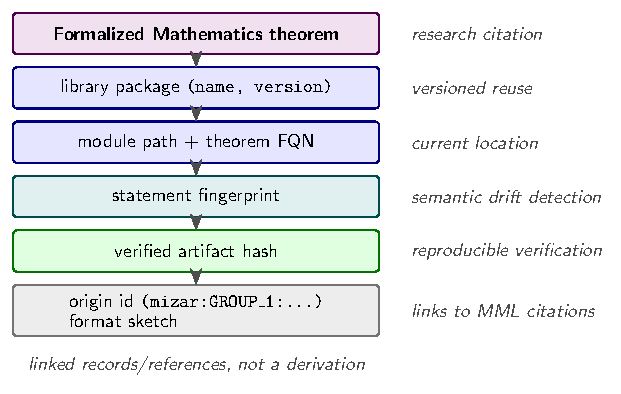
\includegraphics[width=\textwidth,height=0.66\textheight,keepaspectratio]{figures/fm_links.pdf}
\end{center}
\begin{itemize}
\setlength{\itemsep}{1pt}
\setlength{\parsep}{0pt}
\setlength{\parskip}{0pt}
\item This sketch links citations, library items, verification artifacts, and MML origins.
\item It shows links between records, not a derivation.
\end{itemize}
\note{
\smallskip
\textbf{Read aloud:}
\begin{itemize}
\setlength{\itemsep}{1pt}
\setlength{\parsep}{0pt}
\setlength{\parskip}{0pt}
\item This sketch links citations, library items, verification artifacts, and MML origins.
\item It shows links between records, not a derivation.
\end{itemize}
}
\end{frame}

\begin{frame}[fragile,t]{9.3 - Who Gains What\deepdivetag}
\begin{footnotesize}
\setlength{\tabcolsep}{3pt}
\renewcommand{\arraystretch}{1.15}
\begin{tabularx}{\textwidth}{>{\raggedright\arraybackslash}X>{\raggedright\arraybackslash}X}
\toprule
\textbf{Audience} & \textbf{Gain} \\
\midrule
readers & written explanations come first; formal source is one click away \\
maintainers & refactoring no longer rewrites published explanations \\
authors & frozen \texttt{pub} article identities; FQNs for library locations \\
planned AI tools & prose for retrieval, fingerprints for exact context \\
\bottomrule
\end{tabularx}
\end{footnotesize}

\note{
Optional detail (see slide).

}
\end{frame}

\begin{frame}[fragile,t]{9.4 - What Is Preserved, What We Ask}
\begin{itemize}
\setlength{\itemsep}{1pt}
\setlength{\parsep}{0pt}
\setlength{\parskip}{0pt}
\item Formalized Mathematics would remain a journal with review and written explanations.
\item Origin metadata would link migrated items to their MML citations. The migration mapping still needs to be defined.
\item I would like to discuss which identifiers readers should see in citations.
\item That completes the eight stories. Let us now look at the whole design.
\end{itemize}
\smallskip
\textbf{Questions for later review:}
\begin{itemize}
\setlength{\itemsep}{1pt}
\setlength{\parsep}{0pt}
\setlength{\parskip}{0pt}
\item Which identity should be primary in user-facing citations: article label, library FQN, or origin id?
\item How should existing Formalized Mathematics articles link to migrated modules - by updating old links now, when articles are revised, or not at all?
\end{itemize}
\note{
\smallskip
\textbf{Read aloud:}
\begin{itemize}
\setlength{\itemsep}{1pt}
\setlength{\parsep}{0pt}
\setlength{\parskip}{0pt}
\item Formalized Mathematics would remain a journal with review and written explanations.
\item Origin metadata would link migrated items to their MML citations. The migration mapping still needs to be defined.
\item I would like to discuss which identifiers readers should see in citations.
\item That completes the eight stories. Let us now look at the whole design.
\end{itemize}
}
\end{frame}

\section{Part 10. Architecture In One Picture}
\begin{frame}[fragile,t]{10.1 - The Core ATP Path}
\begin{center}
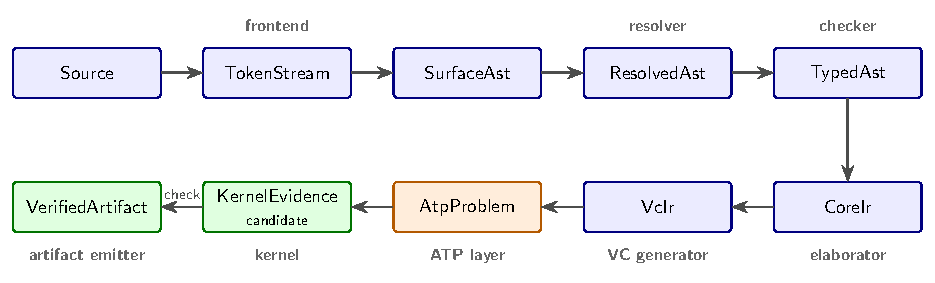
\includegraphics[width=\textwidth,height=0.52\textheight,keepaspectratio]{figures/pipeline.pdf}
\end{center}
\begin{itemize}
\setlength{\itemsep}{1pt}
\setlength{\parsep}{0pt}
\setlength{\parskip}{0pt}
\item This diagram shows the ATP path through the proposed pipeline.
\item Only obligations still open after deterministic discharge go to ATP. Earlier discharge also needs evidence.
\item Each boundary states who owns a fact, which artifact records it, and what must be checked again after a change.
\end{itemize}
\note{
\smallskip
\textbf{Read aloud:}
\begin{itemize}
\setlength{\itemsep}{1pt}
\setlength{\parsep}{0pt}
\setlength{\parskip}{0pt}
\item This diagram shows the ATP path through the proposed pipeline.
\item Only obligations still open after deterministic discharge go to ATP. Earlier discharge also needs evidence.
\item Each boundary states who owns a fact, which artifact records it, and what must be checked again after a change.
\end{itemize}
}
\end{frame}

\begin{frame}[fragile,t]{10.2 - Responsibility Split\deepdivetag}
\begin{footnotesize}
\setlength{\tabcolsep}{3pt}
\renewcommand{\arraystretch}{1.15}
\begin{tabularx}{\textwidth}{>{\raggedright\arraybackslash}X>{\raggedright\arraybackslash}X}
\toprule
\textbf{Layer} & \textbf{Responsibility} \\
\midrule
frontend & lexing, parsing, recovery \\
resolver & imports, names, labels, namespaces \\
checker & soft types, clusters, registrations, overloads \\
elaborator & core logical representation \\
VC generator & proof and algorithm obligations \\
ATP layer plus kernel & untrusted search, then acceptance by checking \\
artifact emitter & stable outputs for tools and dependents \\
\bottomrule
\end{tabularx}
\end{footnotesize}

\note{
Optional detail (see slide).

}
\end{frame}

\begin{frame}[fragile,t]{10.3 - Pipeline Stages For The Eight Stories}
\begin{itemize}
\setlength{\itemsep}{1pt}
\setlength{\parsep}{0pt}
\setlength{\parskip}{0pt}
\item These eight stories belong to one pipeline, from name resolution to publication.
\item Each stage keeps its own responsibility for meaning and proof checking.
\end{itemize}
\smallskip
\textbf{Details for later review:}
\begin{footnotesize}
\setlength{\tabcolsep}{3pt}
\renewcommand{\arraystretch}{1.15}
\begin{tabularx}{\textwidth}{>{\raggedright\arraybackslash}X>{\raggedright\arraybackslash}X}
\toprule
\textbf{Story} & \textbf{Pipeline stage} \\
\midrule
dependencies & resolver, package manager \\
structures and automation & checker (inheritance and cluster graphs, traces) \\
search vs trust & ATP layer, kernel, formula/substitution evidence \\
scale & artifacts, fingerprints, scheduler \\
templates & elaborator (checked instantiation) \\
algorithms & VC generator, MVM \\
publication & artifact emitter, doc generation \\
\bottomrule
\end{tabularx}
\end{footnotesize}

\note{
\smallskip
\textbf{Read aloud:}
\begin{itemize}
\setlength{\itemsep}{1pt}
\setlength{\parsep}{0pt}
\setlength{\parskip}{0pt}
\item These eight stories belong to one pipeline, from name resolution to publication.
\item Each stage keeps its own responsibility for meaning and proof checking.
\end{itemize}
}
\end{frame}

\begin{frame}[fragile,t]{10.4 - Testing The Trust Boundary\deepdivetag}
\smallskip
\textbf{Key Phrase:}
\begin{center}
\begin{beamercolorbox}[rounded=true,sep=2.5mm,wd=0.9\textwidth]{keyphrase}
\centering\itshape Reject what must not pass\\ before\\ Accept everything that should pass
\end{beamercolorbox}
\end{center}
\smallskip
\textbf{Key Points:}
\begin{itemize}
\setlength{\itemsep}{1pt}
\setlength{\parsep}{0pt}
\setlength{\parskip}{0pt}
\item soundness bugs have higher priority than parser gaps. Tests near the kernel first focus on malformed and failing evidence;
\item with these tests in place, we add coverage for accepted language forms.
\end{itemize}
\note{
\smallskip
\textbf{Read aloud:}
\begin{itemize}
\setlength{\itemsep}{1pt}
\setlength{\parsep}{0pt}
\setlength{\parskip}{0pt}
\item Reject what must not pass before Accept everything that should pass
\item soundness bugs have higher priority than parser gaps. Tests near the kernel first focus on malformed and failing evidence;
\item with these tests in place, we add coverage for accepted language forms.
\end{itemize}
}
\end{frame}

\section{Part 11. Roadmap And Collaboration}
\begin{frame}[fragile,t]{11.0 - Where The Project Stands Today}
\begin{itemize}
\setlength{\itemsep}{1pt}
\setlength{\parsep}{0pt}
\setlength{\parskip}{0pt}
\item Before I finish, let me separate the design from the implementation.
\item The specification has 24 chapters and appendices. English is canonical; Japanese companions are available.
\item Implemented parts include frontend processing, selected semantic cases, ATP candidate generation, and kernel evidence checking.
\item The full path from source through ATP and kernel checking to published artifacts is still in progress. Tests with real external provers are still needed.
\item MVM execution, code extraction, and full MML migration remain future work.
\end{itemize}
\note{
\smallskip
\textbf{Read aloud:}
\begin{itemize}
\setlength{\itemsep}{1pt}
\setlength{\parsep}{0pt}
\setlength{\parskip}{0pt}
\item Before I finish, let me separate the design from the implementation.
\item The specification has 24 chapters and appendices. English is canonical; Japanese companions are available.
\item Implemented parts include frontend processing, selected semantic cases, ATP candidate generation, and kernel evidence checking.
\item The full path from source through ATP and kernel checking to published artifacts is still in progress. Tests with real external provers are still needed.
\item MVM execution, code extraction, and full MML migration remain future work.
\end{itemize}
\smallskip
\textbf{Optional notes and sources:}
\begin{itemize}
\setlength{\itemsep}{1pt}
\setlength{\parsep}{0pt}
\setlength{\parskip}{0pt}
\item This is the September 2026 scope. Component tests do not show that the full pipeline works. See \texttt{doc/design/todo.md}, Completion Gates.
\end{itemize}
}
\end{frame}

\begin{frame}[fragile,t]{11.1 - Migration Needs Research}
\begin{center}
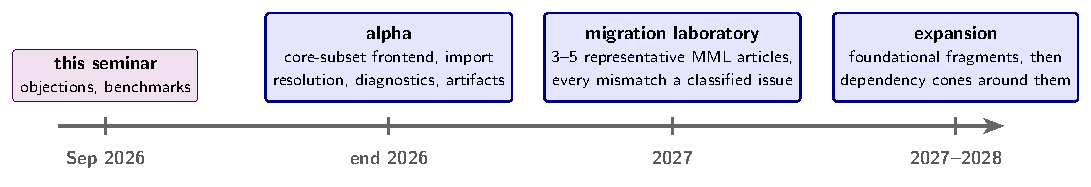
\includegraphics[width=\textwidth,height=0.52\textheight,keepaspectratio]{figures/roadmap_timeline.pdf}
\end{center}
\begin{itemize}
\setlength{\itemsep}{1pt}
\setlength{\parsep}{0pt}
\setlength{\parskip}{0pt}
\item We plan an alpha at the end of 2026. It covers a core frontend subset, import and module resolution prototypes, diagnostics, and early artifacts.
\item In 2027, we plan to translate three to five representative MML articles by hand and by script. We will record every mismatch.
\item In 2027 and 2028, we plan to expand from set and relation fragments to algebraic structures and their dependencies.
\item The alpha does not aim at full MML verification, a final compatibility layer, or a stable AI protocol.
\end{itemize}
\note{
\smallskip
\textbf{Read aloud:}
\begin{itemize}
\setlength{\itemsep}{1pt}
\setlength{\parsep}{0pt}
\setlength{\parskip}{0pt}
\item We plan an alpha at the end of 2026. It covers a core frontend subset, import and module resolution prototypes, diagnostics, and early artifacts.
\item In 2027, we plan to translate three to five representative MML articles by hand and by script. We will record every mismatch.
\item In 2027 and 2028, we plan to expand from set and relation fragments to algebraic structures and their dependencies.
\item The alpha does not aim at full MML verification, a final compatibility layer, or a stable AI protocol.
\end{itemize}
}
\end{frame}

\begin{frame}[fragile,t]{11.2 - What We Will Measure\deepdivetag}
\smallskip
\textbf{Key Points:}
\begin{itemize}
\setlength{\itemsep}{1pt}
\setlength{\parsep}{0pt}
\setlength{\parskip}{0pt}
\item translated articles and lines; accepted parser subset;
\item resolved imports versus unresolved dependencies;
\item obligations closed deterministically versus by ATP with kernel evidence;
\item memory and wall-clock per module, incremental versus clean;
\item compatibility decisions that required human judgment.
\end{itemize}
\note{
\smallskip
\textbf{Read aloud:}
\begin{itemize}
\setlength{\itemsep}{1pt}
\setlength{\parsep}{0pt}
\setlength{\parskip}{0pt}
\item translated articles and lines; accepted parser subset;
\item resolved imports versus unresolved dependencies;
\item obligations closed deterministically versus by ATP with kernel evidence;
\item memory and wall-clock per module, incremental versus clean;
\item compatibility decisions that required human judgment.
\end{itemize}
}
\end{frame}

\begin{frame}[fragile,t]{11.3 - Compatibility Policy And Risks\deepdivetag}
\smallskip
\textbf{Policy:}
\begin{itemize}
\setlength{\itemsep}{1pt}
\setlength{\parsep}{0pt}
\setlength{\parskip}{0pt}
\item define origin mappings to preserve MML theorem identity;
\item keep compatibility aliases where they help migration;
\item record every difference from old behavior with a reason and a test.
\end{itemize}
\begin{footnotesize}
\setlength{\tabcolsep}{3pt}
\renewcommand{\arraystretch}{1.15}
\begin{tabularx}{\textwidth}{>{\raggedright\arraybackslash}X>{\raggedright\arraybackslash}X}
\toprule
\textbf{Risk} & \textbf{How to reduce it} \\
\midrule
compatibility work takes all our time & small representative parts first; no all-at-once translation \\
registrations behave differently & trace artifacts and comparison reports early \\
package layout breaks journal links & origin metadata, article-to-library identifiers \\
AI edits hide migration mistakes & Red edits stay forbidden to ordinary agents; verifier artifacts required \\
\bottomrule
\end{tabularx}
\end{footnotesize}

\note{
\smallskip
\textbf{Read aloud:}
\begin{itemize}
\setlength{\itemsep}{1pt}
\setlength{\parsep}{0pt}
\setlength{\parskip}{0pt}
\item define origin mappings to preserve MML theorem identity;
\item keep compatibility aliases where they help migration;
\item record every difference from old behavior with a reason and a test.
\end{itemize}
}
\end{frame}

\begin{frame}[fragile,t]{11.4 - What September 2026 Should Produce}
\begin{itemize}
\setlength{\itemsep}{1pt}
\setlength{\parsep}{0pt}
\setlength{\parskip}{0pt}
\item For this visit, I hope we can choose migration benchmark articles in priority order.
\item I would like to agree on the compatibility metadata we need.
\item I also hope to collect comments on the eight stories, especially structures and clusters.
\item A first paper outline and a shared list of objections would help guide the next steps.
\end{itemize}
\note{
\smallskip
\textbf{Read aloud:}
\begin{itemize}
\setlength{\itemsep}{1pt}
\setlength{\parsep}{0pt}
\setlength{\parskip}{0pt}
\item For this visit, I hope we can choose migration benchmark articles in priority order.
\item I would like to agree on the compatibility metadata we need.
\item I also hope to collect comments on the eight stories, especially structures and clusters.
\item A first paper outline and a shared list of objections would help guide the next steps.
\end{itemize}
}
\end{frame}

\begin{frame}[fragile,t]{11.5 - What We Ask Of You}
\begin{itemize}
\setlength{\itemsep}{1pt}
\setlength{\parsep}{0pt}
\setlength{\parskip}{0pt}
\item I do not expect us to settle every design question today.
\item The handout keeps the questions below for later review.
\item Your choice of small MML examples would help us test the proposal in practice.
\end{itemize}
\smallskip
\textbf{Questions for later review:}
\begin{itemize}
\setlength{\itemsep}{1pt}
\setlength{\parsep}{0pt}
\setlength{\parskip}{0pt}
\item Which MML articles are small but structurally representative?
\item Which idioms matter to the Mizar community, beyond their technical use?
\item Which of the eight stories is most wrong, and why?
\item What migration result would convince the community that Evo is a serious project?
\end{itemize}
\note{
\smallskip
\textbf{Read aloud:}
\begin{itemize}
\setlength{\itemsep}{1pt}
\setlength{\parsep}{0pt}
\setlength{\parskip}{0pt}
\item I do not expect us to settle every design question today.
\item The handout keeps the questions below for later review.
\item Your choice of small MML examples would help us test the proposal in practice.
\end{itemize}
}
\end{frame}

\section{Part 12. Closing}
\begin{frame}[fragile,t]{12.1 - The Main Question, Again}
\begin{itemize}
\setlength{\itemsep}{1pt}
\setlength{\parsep}{0pt}
\setlength{\parskip}{0pt}
\item I would like to finish with the question from the beginning.
\end{itemize}
\smallskip
\textbf{Slide question:}
\begin{center}
\begin{beamercolorbox}[rounded=true,sep=2.5mm,wd=0.9\textwidth]{keyphrase}
\centering\itshape What must Mizar Evo preserve so that the Mizar community\\ still recognizes it as Mizar?
\end{beamercolorbox}
\end{center}
\begin{itemize}
\setlength{\itemsep}{1pt}
\setlength{\parsep}{0pt}
\setlength{\parskip}{0pt}
\item Which small MML articles should we migrate first?
\item Which proposal needs the most change?
\end{itemize}
\note{
\smallskip
\textbf{Read aloud:}
\begin{itemize}
\setlength{\itemsep}{1pt}
\setlength{\parsep}{0pt}
\setlength{\parskip}{0pt}
\item I would like to finish with the question from the beginning.
\item What must Mizar Evo preserve so that the Mizar community still recognizes it as Mizar?
\item Which small MML articles should we migrate first?
\item Which proposal needs the most change?
\end{itemize}
}
\end{frame}

\begin{frame}[fragile,t]{12.2 - Closing}
\begin{itemize}
\setlength{\itemsep}{1pt}
\setlength{\parsep}{0pt}
\setlength{\parskip}{0pt}
\item Mizar Evo should update the parts that need to support a larger library.
\item It should keep the parts that define Mizar's mathematical identity.
\item Thank you for listening. I would welcome your questions and comments.
\end{itemize}
\note{
\smallskip
\textbf{Read aloud:}
\begin{itemize}
\setlength{\itemsep}{1pt}
\setlength{\parsep}{0pt}
\setlength{\parskip}{0pt}
\item Mizar Evo should update the parts that need to support a larger library.
\item It should keep the parts that define Mizar's mathematical identity.
\item Thank you for listening. I would welcome your questions and comments.
\end{itemize}
}
\end{frame}

\appendix
\section{Backup A. Prepared Exact Examples}
\begin{frame}[fragile,t]{Backup A. Prepared Exact Examples (1/2)}
\smallskip
\textbf{Exact excerpts used in this talk:}
\begin{scriptsize}
\setlength{\tabcolsep}{3pt}
\renewcommand{\arraystretch}{1.15}
\begin{tabularx}{\textwidth}{>{\raggedright\arraybackslash}X>{\raggedright\arraybackslash}X>{\raggedright\arraybackslash}X>{\raggedright\arraybackslash}X}
\toprule
\textbf{Purpose} & \textbf{Source} & \textbf{Lines} & \textbf{Used in} \\
\midrule
Structure definition & \texttt{algstr\_0.miz} & 37-40 & Frames 0.2, 3.1 \\
Article environment & \texttt{algstr\_0.miz} & 15-25 & Frame 2.1 \\
Registration/cluster & \texttt{algstr\_0.miz} & 104-109 & Frame 4.1 \\
\bottomrule
\end{tabularx}
\end{scriptsize}

\smallskip
\textbf{Exact excerpts used in this talk:}
\begin{scriptsize}
\setlength{\tabcolsep}{3pt}
\renewcommand{\arraystretch}{1.15}
\begin{tabularx}{\textwidth}{>{\raggedright\arraybackslash}X>{\raggedright\arraybackslash}X>{\raggedright\arraybackslash}X>{\raggedright\arraybackslash}X}
\toprule
\textbf{Purpose} & \textbf{Source} & \textbf{Lines} & \textbf{Used in} \\
\midrule
Proof citation & \texttt{struct\_0.miz} & 637-643 & Frame 5.4 \\
Induction scheme & \texttt{nat\_1.miz} & near 90 & Frame 7.1 \\
\bottomrule
\end{tabularx}
\end{scriptsize}

\smallskip
\textbf{Source URLs:}
\begin{itemize}
\setlength{\itemsep}{1pt}
\setlength{\parsep}{0pt}
\setlength{\parskip}{0pt}
\item \texttt{ALGSTR\_0}: \url{https://mizar.uwb.edu.pl/version/current/mml/algstr\_0.miz}
\item \texttt{STRUCT\_0}: \url{https://mizar.uwb.edu.pl/version/current/mml/struct\_0.miz}
\item \texttt{NAT\_1}: \url{https://mizar.uwb.edu.pl/version/current/mml/nat\_1.miz}
\end{itemize}
\note{
\smallskip
\textbf{Read aloud:}
\begin{itemize}
\setlength{\itemsep}{1pt}
\setlength{\parsep}{0pt}
\setlength{\parskip}{0pt}
\item \texttt{ALGSTR\_0}: \url{https://mizar.uwb.edu.pl/version/current/mml/algstr\_0.miz}
\item \texttt{STRUCT\_0}: \url{https://mizar.uwb.edu.pl/version/current/mml/struct\_0.miz}
\item \texttt{NAT\_1}: \url{https://mizar.uwb.edu.pl/version/current/mml/nat\_1.miz}
\end{itemize}
}
\end{frame}

\begin{frame}[fragile,t]{Backup A. Prepared Exact Examples (2/2)}
\smallskip
\textbf{Attribution note:}
\begin{itemize}
\setlength{\itemsep}{1pt}
\setlength{\parsep}{0pt}
\setlength{\parskip}{0pt}
\item MML plain-text files state GPL-3.0-or-later / CC-BY-SA-3.0-or-later terms; keep article attribution, URLs, and line numbers in speaker notes.
\end{itemize}
\note{
\smallskip
\textbf{Read aloud:}
\begin{itemize}
\setlength{\itemsep}{1pt}
\setlength{\parsep}{0pt}
\setlength{\parskip}{0pt}
\item MML plain-text files state GPL-3.0-or-later / CC-BY-SA-3.0-or-later terms; keep article attribution, URLs, and line numbers in speaker notes.
\end{itemize}
}
\end{frame}

\section{Backup B. Specification Reference Map}
\begin{frame}[fragile,t]{Backup B. Specification Reference Map (1/2)}
Specification used: 10 September 2026. For grammar and semantics, see \texttt{doc/spec/en/00.index.md} in the repository (\url{https://github.com/aabaa/mizar-evo}). Online files may change after this talk.

\begin{footnotesize}
\setlength{\tabcolsep}{3pt}
\renewcommand{\arraystretch}{1.15}
\begin{tabularx}{\textwidth}{>{\raggedright\arraybackslash}X>{\raggedright\arraybackslash}X}
\toprule
\textbf{Topic} & \textbf{Specification source (under \texttt{doc/spec/en/})} \\
\midrule
Modules and imports & \texttt{12.modules\_and\_namespaces.md} \\
Structures and inheritance & \texttt{05.structures.md} \\
Attributes and modes & \texttt{06.attributes.md}, \texttt{07.modes.md} \\
Registrations and reductions & \texttt{17.clusters\_and\_registrations.md} \\
Templates and schemes & \texttt{18.templates.md} \\
Algorithms and MVM & \texttt{20.algorithm\_and\_verification.md} \\
ATP and kernel evidence & \texttt{21.source\_code\_annotation\_and\_atp.md} \\
\bottomrule
\end{tabularx}
\end{footnotesize}

\note{
\smallskip
\textbf{Read aloud:}
\begin{itemize}
\setlength{\itemsep}{1pt}
\setlength{\parsep}{0pt}
\setlength{\parskip}{0pt}
\item Specification used: 10 September 2026. For grammar and semantics, see \texttt{doc/spec/en/00.index.md} in the repository (\url{https://github.com/aabaa/mizar-evo}). Online files may change after this talk.
\end{itemize}
}
\end{frame}

\begin{frame}[fragile,t]{Backup B. Specification Reference Map (2/2)}
\begin{footnotesize}
\setlength{\tabcolsep}{3pt}
\renewcommand{\arraystretch}{1.15}
\begin{tabularx}{\textwidth}{>{\raggedright\arraybackslash}X>{\raggedright\arraybackslash}X}
\toprule
\textbf{Topic} & \textbf{Specification source (under \texttt{doc/spec/en/})} \\
\midrule
Packages and artifacts & \texttt{23.package\_management\_and\_build\_system.md} \\
Cross-chapter grammar & \texttt{appendix\_a.grammar\_summary.md} \\
Worked library sketches & \texttt{sample\_codes.md} \\
\bottomrule
\end{tabularx}
\end{footnotesize}

\note{
Optional detail (see slide).

}
\end{frame}

\section{Backup D. Possible Paper Outline}
\begin{frame}[fragile,t]{Backup D. Possible Paper Outline (1/2)}
\smallskip
\textbf{Possible paper title:}
\begin{center}
\begin{beamercolorbox}[rounded=true,sep=2.5mm,wd=0.9\textwidth]{keyphrase}
\centering\itshape Mizar Evo: Readable, AI-Ready, and Scalable Formal Mathematics
\end{beamercolorbox}
\end{center}
\smallskip
\textbf{Possible sections:}
\begin{enumerate}
\setlength{\itemsep}{1pt}
\setlength{\parsep}{0pt}
\setlength{\parskip}{0pt}
\item Introduction: why Mizar needs evolution now.
\item Mizar as baseline: readability, MML, Formalized Mathematics.
\item Design principles and the three goals.
\item Language evolution: dependencies, structures, registrations, templates.
\item Verifier architecture, kernel evidence, and the trusted SAT checker.
\item Verified computation and the MVM.
\item AI-safe proof development.
\end{enumerate}
\note{
\smallskip
\textbf{Read aloud:}
\begin{itemize}
\setlength{\itemsep}{1pt}
\setlength{\parsep}{0pt}
\setlength{\parskip}{0pt}
\item Mizar Evo: Readable, AI-Ready, and Scalable Formal Mathematics
\item Introduction: why Mizar needs evolution now.
\item Mizar as baseline: readability, MML, Formalized Mathematics.
\item Design principles and the three goals.
\item Language evolution: dependencies, structures, registrations, templates.
\item Verifier architecture, kernel evidence, and the trusted SAT checker.
\item Verified computation and the MVM.
\item AI-safe proof development.
\end{itemize}
}
\end{frame}

\begin{frame}[fragile,t]{Backup D. Possible Paper Outline (2/2)}
\smallskip
\textbf{Possible sections:}
\begin{enumerate}
\setlength{\itemsep}{1pt}
\setlength{\parsep}{0pt}
\setlength{\parskip}{0pt}
\item Package-based library and publication workflow.
\item Migration plan and evaluation measures.
\item Related work and plans for working together.
\end{enumerate}
\note{
\smallskip
\textbf{Read aloud:}
\begin{itemize}
\setlength{\itemsep}{1pt}
\setlength{\parsep}{0pt}
\setlength{\parskip}{0pt}
\item Package-based library and publication workflow.
\item Migration plan and evaluation measures.
\item Related work and plans for working together.
\end{itemize}
}
\end{frame}

\section{Backup F. Possible Objections}
\begin{frame}[fragile,t]{Backup F. Possible Objections (1/2)}
\smallskip
\textbf{Prepared answers to other possible objections:}
\begin{footnotesize}
\setlength{\tabcolsep}{3pt}
\renewcommand{\arraystretch}{1.15}
\begin{tabularx}{\textwidth}{>{\raggedright\arraybackslash}X>{\raggedright\arraybackslash}X}
\toprule
\textbf{Objection} & \textbf{Prepared answer} \\
\midrule
Why not improve current Mizar incrementally? & Some proposals may also help existing tools. Evo explores changes to modules, proof evidence, and library artifacts together. Migration examples should help us decide which changes are useful. \\
What happens to authorship and credit of MML articles? & We propose origin mappings that preserve identity and credit during migration. The mapping format is still open. The \texttt{pub} namespace keeps published articles unchanged. \\
Is this a fork of the community? & It is a proposal to the community; this visit is its first review. The namespace governance model assumes that the Mizar team controls the \texttt{mml} root. \\
\bottomrule
\end{tabularx}
\end{footnotesize}

\note{
Optional detail (see slide).

\smallskip
\textbf{Optional notes and sources:}
\begin{itemize}
\setlength{\itemsep}{1pt}
\setlength{\parsep}{0pt}
\setlength{\parskip}{0pt}
\item Use these answers only if someone asks these questions.
\end{itemize}
}
\end{frame}

\begin{frame}[fragile,t]{Backup F. Possible Objections (2/2)}
\smallskip
\textbf{Prepared answers to other possible objections:}
\begin{footnotesize}
\setlength{\tabcolsep}{3pt}
\renewcommand{\arraystretch}{1.15}
\begin{tabularx}{\textwidth}{>{\raggedright\arraybackslash}X>{\raggedright\arraybackslash}X}
\toprule
\textbf{Objection} & \textbf{Prepared answer} \\
\midrule
What about GPL / CC-BY-SA obligations? & Migration preserves license and attribution of MML content; toolchain licensing is open for discussion. \\
Are the claims about AI too strong? & AI assistance is an optional layer that never enters the trusted base; every proposal also works without it. \\
Why a new kernel instead of the existing checker? & Formula/substitution evidence needs a small trusted core, including a SAT checker. Mizar Evo's specification defines the obligations; legacy behavior guides migration comparisons. \\
\bottomrule
\end{tabularx}
\end{footnotesize}

\note{
Optional detail (see slide).

}
\end{frame}

\end{document}
